\documentclass[11pt,a4paper]{article}

% Packages
\usepackage[utf8]{inputenc}
\usepackage{csvsimple}
\usepackage[T1]{fontenc}
\usepackage{times}
\usepackage[margin=1in]{geometry}
\usepackage{graphicx}
\usepackage{booktabs}
\usepackage{multirow}
\usepackage{array}
\usepackage{longtable}
\usepackage{hyperref}
\usepackage{xcolor}
\usepackage{float}
\usepackage{caption}
\usepackage{subcaption}
\usepackage[numbers,sort&compress]{natbib}
\usepackage{setspace}
\usepackage{enumitem}
\usepackage{pdflscape}
\usepackage{ltablex}
\usepackage{xstring}
\usepackage{newunicodechar}
\usepackage{amssymb}

% Unicode character mappings for the imported dataset table
\newunicodechar{∗}{*}
\newunicodechar{⋆}{*}
\newunicodechar{†}{\textdagger}
\newunicodechar{‡}{\textdaggerdbl}
\newunicodechar{fi}{fi}
\newunicodechar{fl}{fl}
\newunicodechar{ţ}{\c{t}}
\newunicodechar{ć}{\'c}
\newunicodechar{•}{\textbullet}
\newunicodechar{ℎ}{h}
\newunicodechar{∥}{\ensuremath{\parallel}}
\newunicodechar{≀}{\ensuremath{\wr}}
\newunicodechar{§}{\S}
\newunicodechar{¶}{\P}
\newunicodechar{ß}{\ss}
\newunicodechar{à}{\`a}
\newunicodechar{ä}{\"a}
\newunicodechar{è}{\`e}
\newunicodechar{ö}{\"o}
\newunicodechar{ü}{\"u}
\newunicodechar{⇤}{<-}
\newunicodechar{​}{} % zero-width non-joiner
% Math bold/italic letters normalized to ASCII
\newunicodechar{𝐵}{B}
\newunicodechar{𝐻}{H}
\newunicodechar{𝑆}{S}
\newunicodechar{𝑊}{W}
\newunicodechar{𝑌}{Y}
\newunicodechar{𝑍}{Z}
\newunicodechar{𝑎}{a}
\newunicodechar{𝑔}{g}
\newunicodechar{𝑖}{i}
\newunicodechar{𝑛}{n}
\newunicodechar{𝑜}{o}
\newunicodechar{𝑢}{u}
\newunicodechar{𝑳}{L}
\newunicodechar{𝑵}{N}
\newunicodechar{𝑺}{S}
\newunicodechar{𝒂}{a}
\newunicodechar{𝒃}{b}
\newunicodechar{𝒅}{d}
\newunicodechar{𝒆}{e}
\newunicodechar{𝒉}{h}
\newunicodechar{𝒊}{i}
\newunicodechar{𝒌}{k}
\newunicodechar{𝒍}{l}
\newunicodechar{𝒐}{o}
\newunicodechar{𝒓}{r}
\newunicodechar{𝒔}{s}
\newunicodechar{𝒚}{y}
\newunicodechar{𝟏}{1}
\newcommand{\yn}[1]{\IfStrEq{#1}{YES}{\checkmark}{\IfStrEq{#1}{NO}{\(\times\)}{\IfStrEq{#1}{~}{\textit{n/a}}{#1}}}}
\newcommand{\threat}[1]{\IfStrEq{#1}{White-box}{W}{\IfStrEq{#1}{Black-box}{B}{\IfStrEq{#1}{Gray-box}{G}{\IfStrEq{#1}{Partial}{P}{#1}}}}}
\newcommand{\access}[1]{\IfStrEq{#1}{Full}{F}{\IfStrEq{#1}{Partial}{P}{\IfStrEq{#1}{~}{\textit{n/a}}{#1}}}}
\newcommand{\level}[1]{\IfStrEq{#1}{High}{H}{\IfStrEq{#1}{Low}{L}{\IfStrEq{#1}{~}{\textit{n/a}}{#1}}}}

% Narrow column helper for wide tables
\newcolumntype{Y}{>{\centering\arraybackslash}p{0.9cm}}
\keepXColumns

% Hyperref setup
\hypersetup{
    colorlinks=true,
    linkcolor=blue,
    citecolor=blue,
    urlcolor=blue
}

% Line spacing
\onehalfspacing

% Title
\title{\textbf{Bridging the Gap Between Theory and Practice in Adversarial Machine Learning: A Systematic Cross-Venue Analysis of 454 Papers (2022--2025)}}

\author{
  Madhav Khanal\\
  Rollins College\\
  \texttt{mkhanal@rollins.edu}
  \and
  JJ Jasser\\
  Rollins College\\
  \texttt{jjasser@rollins.edu}
}

\date{}

\begin{document}

\maketitle

%==============================================================================
% ABSTRACT
%==============================================================================
\begin{abstract}
Machine learning systems are increasingly deployed in security-critical contexts, yet the gap between academic adversarial machine learning research and practical security needs remains substantial. This systematic review analyzes 454 papers published from 2022 to 2025 across four leading security conferences (ACM CCS, IEEE S\&P, NDSS, and USENIX Security), applying a framework adapted from Apruzzese et\,al.\ to evaluate how well current work addresses real-world deployment constraints. Our analysis reveals that only 5.3\% of papers evaluate methods on deployed systems, while 67.8\% rely on gradient access and 63.2\% assume white-box threat models. We identify five dimensions requiring greater attention: realistic threat modeling, constrained attacker knowledge, validation on production systems, diversification beyond computer vision, and consideration of economic and human factors. We further examine emerging challenges posed by large language models and document real-world adversarial incidents that illustrate the sociotechnical nature of ML security threats. Based on these findings, we offer recommendations for researchers, conference organizers, practitioners, and funding agencies to better align adversarial ML research with operational security requirements.

\textbf{Keywords:} adversarial machine learning, theory-practice gap, security research, systematic review, threat modeling
\end{abstract}

\newpage
\tableofcontents
\newpage

%==============================================================================
% 1. INTRODUCTION
%==============================================================================
\section{Introduction}

Machine learning has become integral to software systems across numerous domains. Applications range from facial recognition at border crossings and fraud detection in financial services to navigation for autonomous vehicles and content moderation on social platforms. Large language models now power customer service chatbots, code generation tools, and medical decision support systems. These models influence decisions affecting millions of people daily, prompting increased scrutiny of their vulnerabilities. Researchers have demonstrated that carefully crafted inputs can trigger failures in ML systems that designers did not anticipate.

The field of adversarial machine learning (AML) has emerged to study these weaknesses and develop countermeasures. Over the past decade, researchers have demonstrated diverse attack vectors: imperceptible perturbations causing image misclassification, poisoned training data implanting hidden backdoors, and privacy attacks extracting sensitive information through query access. The community has proposed numerous defenses to strengthen models against such threats.

Despite these advances, a fundamental question persists: \textbf{How well do the assumptions underlying academic research correspond to the constraints of deployed systems?}

In 2023, Apruzzese and colleagues published an influential analysis titled ``Real Attackers Don't Compute Gradients''~\citep{apruzzese2022real}, documenting a significant gap between academic AML research and practical security requirements. Their central observation was that academic studies frequently assume attackers can compute gradients of target models, requiring complete access to model internals, whereas real-world attackers typically lack such access. Moreover, simpler methods such as social engineering or basic input manipulation often suffice for malicious purposes, rendering elaborate gradient-based techniques unnecessary outside laboratory settings.

This systematic review investigates how the research community has responded since this critique. We analyzed 454 adversarial ML papers published from 2022 through 2025 in four top-tier security venues: ACM CCS (118 papers), IEEE S\&P (79 papers), NDSS (49 papers), and USENIX Security (208 papers). Each paper was evaluated on dimensions related to practical relevance: threat model realism, computational and knowledge assumptions about adversaries, evaluation methodology, and awareness of deployment challenges.

Our findings indicate that the theory-practice gap persists, though encouraging progress is evident in some areas. While research has advanced our technical understanding of adversarial phenomena, many studies continue to explore attacks and defenses under idealized conditions that may not translate to operational settings. This review characterizes the current state of the field, identifies patterns across venues, and provides actionable recommendations for stakeholders seeking to align adversarial ML research with real-world security needs.

%==============================================================================
% 2. BACKGROUND
%==============================================================================
\section{Background: Foundations of Adversarial Machine Learning}

\subsection{The Discovery of Adversarial Vulnerabilities}

The modern study of adversarial machine learning began with the work of Szegedy et al.~\citep{szegedy2013intriguing}, who demonstrated that small, nearly imperceptible modifications to inputs could cause state-of-the-art deep learning models to produce incorrect outputs with high confidence. These were not random errors but systematic vulnerabilities: adversarial examples crafted for one model frequently transferred to independently trained models. This transferability property revealed fundamental limitations in how neural networks generalize and catalyzed widespread interest in adversarial phenomena.

Goodfellow et al.~\citep{goodfellow2014explaining} attributed these vulnerabilities to the linear behavior of neural networks in high-dimensional spaces, rather than to nonlinearity or overfitting as initially hypothesized. They introduced the Fast Gradient Sign Method (FGSM), which generates adversarial inputs efficiently using a single gradient computation. FGSM's simplicity and effectiveness established gradient-based perturbation as the dominant paradigm for evaluating model robustness.

These foundational studies established three conventions that continue to shape adversarial ML research. First, they assumed white-box access to models, providing complete knowledge of architecture and parameters to enable direct gradient computation. Second, they focused on perturbations bounded by specific norm constraints to maintain near-imperceptibility. Third, they framed adversarial example generation as an optimization problem amenable to gradient-based solutions. While these assumptions enabled systematic investigation, they also began to diverge from the conditions under which practical attacks occur.

\subsection{The Arms Race: Attacks and Defenses}

The discovery of adversarial vulnerabilities initiated an ongoing cycle of defenses and adaptive attacks. This dynamic, characterized as an ``arms race'' between attackers and defenders~\citep{carlini2019evaluating}, has defined much of the field's trajectory. Each defense proposal has prompted development of attacks to circumvent it, which in turn has inspired new defensive strategies.

A core challenge in adversarial attack design involves balancing two competing objectives: maximizing classification error while minimizing perturbation visibility. Researchers formalized this as constrained optimization using $L_p$ norms to quantify deviation from original inputs:

\begin{itemize}[noitemsep]
    \item \textbf{$L_0$ norm} counts the number of modified features. An $L_0$ attack might alter few pixels but by substantial amounts.
    \item \textbf{$L_2$ norm} (Euclidean distance) measures root-mean-square difference, distributing small changes across many features.
    \item \textbf{$L_\infty$ norm} bounds the maximum change to any single feature, limiting the conspicuousness of individual modifications.
\end{itemize}

Understanding these metrics is essential because defenses effective against one norm may remain vulnerable to others.

Building on FGSM, researchers developed more sophisticated attack algorithms. Moosavi-Dezfooli et al.~\citep{moosavi2016deepfool} introduced DeepFool, which finds minimal perturbations to cross decision boundaries by iteratively approximating these boundaries as locally linear. Carlini and Wagner~\citep{carlini2017towards} developed optimization-based attacks (C\&W) that minimize a weighted combination of perturbation magnitude and classification error, achieving state-of-the-art success rates across multiple norms. Notably, C\&W attacks defeated defensive distillation~\citep{papernot2016distillation}, demonstrating that gradient obfuscation provides inadequate security.

The iterative defeat of defenses established important evaluation principles. Carlini and Wagner~\citep{carlini2017detecting} systematically evaluated ten detection methods and found all could be circumvented by adaptive adversaries. Athalye et al.~\citep{athalye2018obfuscated} identified ``obfuscated gradients'' as a common but flawed defense strategy, introducing techniques such as Backward Pass Differentiable Approximation (BPDA) to circumvent gradient masking. Their work, which defeated seven of nine defenses accepted to ICLR 2018, established that defenses must be evaluated against adaptive attacks aware of the defense mechanism.

Tramer et al.~\citep{tramer2020adaptive} reinforced this lesson by defeating all thirteen defenses analyzed from top venues that claimed robustness even to adaptive attacks. These results underscore that robust evaluation requires assuming adversaries will adapt their methods to the specific defense deployed.

Two principled approaches emerged from these findings. \textbf{Adversarial training}~\citep{madry2018towards} incorporates adversarial examples into training through min-max optimization:
\[
\min_{\theta} \;\mathbb{E}_{(x,y) \sim D} \Big[ \max_{\|\delta\| \leq \epsilon} \mathcal{L}(f_{\theta}(x + \delta), y) \Big]
\]
This formulation, known as PGD-based adversarial training, remains among the most effective empirical defenses, though it incurs accuracy costs on clean data~\citep{tsipras2019robustness, zhang2019tradeoff}.

\textbf{Certified defenses} provide mathematical guarantees within specified threat models~\citep{li2020sok}. Randomized smoothing~\citep{cohen2019certified} produces provably robust classifiers for $L_2$ perturbations, while interval bound propagation~\citep{gowal2018effectiveness} computes output bounds through network layers. These methods trade computational cost and model flexibility for formal guarantees.

For standardized evaluation, Croce and Hein~\citep{croce2020reliable} introduced AutoAttack, an ensemble of complementary attacks that provides reliable robustness assessment without hyperparameter tuning. The accompanying RobustBench benchmark~\citep{croce2021robustbench} maintains leaderboards across datasets and threat models, enabling consistent comparison of defense methods.

\subsection{Expanding Threat Landscape}

Research has expanded beyond test-time evasion to encompass threats throughout the ML pipeline. \textbf{Membership inference attacks}~\citep{shokri2017membership, ye2021enhanced} determine whether specific samples appeared in training data, potentially violating privacy. Carlini et al.~\citep{carlini2022membership} argued that such attacks should be evaluated at extremely low false-positive rates, since even rare incorrect inferences can cause privacy harm.

\textbf{Training-time attacks} compromise models during development. In \textbf{backdoor attacks}, adversaries introduce trigger patterns causing models to misclassify inputs containing the trigger while behaving normally otherwise~\citep{gu2017badnets}. Recent work has extended backdoors to self-supervised learning~\citep{jia2021badencoder} and developed techniques for inconspicuous poisoned data~\citep{tao2024distribution}. More broadly, \textbf{poisoning attacks} inject corrupted samples to distort model behavior or degrade accuracy~\citep{tramer2022truth}.

\textbf{Physical-world attacks} adapt adversarial examples for real-world conditions including varying angles, lighting, and sensor characteristics. Kurakin et al.~\citep{kurakin2016adversarial} demonstrated that adversarial images remain effective when printed and recaptured by cameras. Jia et al.~\citep{jia2022physical} created adversarial stop signs that fooled autonomous driving systems under realistic conditions. While these results demonstrate feasibility of physical attacks, they also raise questions about whether adversaries would choose such technically demanding approaches when simpler alternatives exist.

\subsection{The Theory-Practice Gap}

Concerns about practical relevance intensified as research became increasingly abstract and benchmark-driven. Kumar et al.~\citep{kumar2020adversarial} interviewed professionals at 28 organizations and found widespread uncertainty about assessing adversarial risks or deploying defenses. Grosse et al.~\citep{grosse2024practical} surveyed 271 industry practitioners, finding that while academic attack scenarios were theoretically possible, researchers frequently overestimated realistic attacker capabilities.

Mink et al.~\citep{mink2023barriers} identified organizational barriers to defense deployment through interviews with ML engineers, documenting unclear responsibility allocation, insufficient incentives for prioritizing robustness, and difficulty integrating adversarial testing into development workflows. Arp et al.~\citep{arp2022dos} conducted a meta-analysis revealing that security research frequently employs simplified laboratory setups that inadequately account for adaptive adversaries or realistic constraints.

Apruzzese et al.~\citep{apruzzese2022real} crystallized these concerns through case studies of actual ML attacks, observing that real incidents typically involved straightforward tactics rather than elaborate gradient-based attacks. Attackers rarely possessed internal model access; instead, they exploited system weaknesses, integration flaws, and human factors. This analysis motivates our systematic examination of whether subsequent research has moved toward addressing practical security needs.

\subsection{Types of Adversarial Attacks}

Adversarial attacks can be categorized by timing and objectives~\citep{biggio2018wild}:

\textbf{Evasion attacks} occur at inference time, manipulating inputs to cause misclassification~\citep{szegedy2013intriguing, goodfellow2014explaining}. These have received the most research attention, though their prevalence in practice remains unclear.

\textbf{Poisoning attacks} occur during training, introducing malicious data to influence model behavior~\citep{biggio2012poisoning}. Backdoor attacks represent a specific variant embedding trigger-activated misbehavior~\citep{gu2017badnets}.

\textbf{Privacy attacks} extract sensitive information from trained models. Membership inference determines training set membership~\citep{shokri2017membership, carlini2022membership}. Model extraction replicates model functionality through queries~\citep{tramer2016stealing, jagielski2020high}. Data reconstruction attempts to recover training samples~\citep{carlini2021extracting}.

\subsection{Threat Models and Their Implications}

Threat model specification is fundamental to security research~\citep{carlini2019evaluating}. In adversarial ML, threat models primarily differ by adversary knowledge:

\textbf{White-box} models assume complete information including architecture, parameters, and potentially training data. This worst-case scenario enables gradient computation and has dominated foundational research.

\textbf{Black-box} models assume query-only access returning predictions or confidence scores~\citep{papernot2017practical}. Attackers must use strategies such as training surrogate models or exploiting transferability.

\textbf{Gray-box} models assume partial knowledge, such as architecture without weights or access to similar training data.

Additional dimensions include query budgets, perturbation constraints, and success criteria. Apruzzese et al.~\citep{apruzzese2022real} emphasized that academic research frequently assumes unrealistically powerful adversaries, while Grosse et al.~\citep{grosse2024practical} found practitioners more concerned with realistic threat models than worst-case $L_p$-bounded perturbations.

%==============================================================================
% 3. REAL-WORLD ADVERSARIAL INCIDENTS
%==============================================================================
\section{Real-World Adversarial Incidents}

It is instructive to consider real examples of adversarial attacks ``in the wild.'' These incidents illustrate the complexity and sociotechnical nature of adversarial misuse and motivate the need to bridge theory and practice. In each case, adversaries exploited system integrations, human behavior, or unanticipated input channels rather than computing optimal perturbations.

\subsection{Case Study: Agentic Use of Frontier LLMs in a State-Sponsored Cyber Campaign}

In November 2025, Anthropic publicly disclosed what it assessed with high confidence to be the first documented large-scale cyber espionage campaign executed predominantly by an AI agent rather than human operators~\citep{anthropic2025ai}. According to the report, a Chinese state-sponsored threat actor manipulated Anthropic's Claude Code system into autonomously conducting cyber operations against approximately thirty global targets, including technology firms, financial institutions, chemical manufacturers, and government agencies.

Crucially, Claude was not used merely as an advisory tool. Instead, the attackers constructed an autonomous attack framework in which the model executed reconnaissance, vulnerability analysis, exploit generation, credential harvesting, and data exfiltration with only intermittent human oversight. Anthropic estimates that the AI system performed approximately 80--90\% of the operational workload, with human operators intervening at a small number of critical decision points~\citep{anthropic2025ai}.

The attack relied on three developments that are largely absent from traditional adversarial ML threat models. First, agentic execution enabled Claude to operate in long-running loops, chaining actions and decisions without constant supervision. Second, tool access via the Model Context Protocol allowed the model to invoke external software such as network scanners and password-cracking utilities. Third, the attackers successfully jailbroke the system's safeguards by decomposing malicious objectives into narrowly scoped, seemingly benign subtasks and framing the activity as legitimate defensive testing.

\begin{figure}[H]
    \centering
    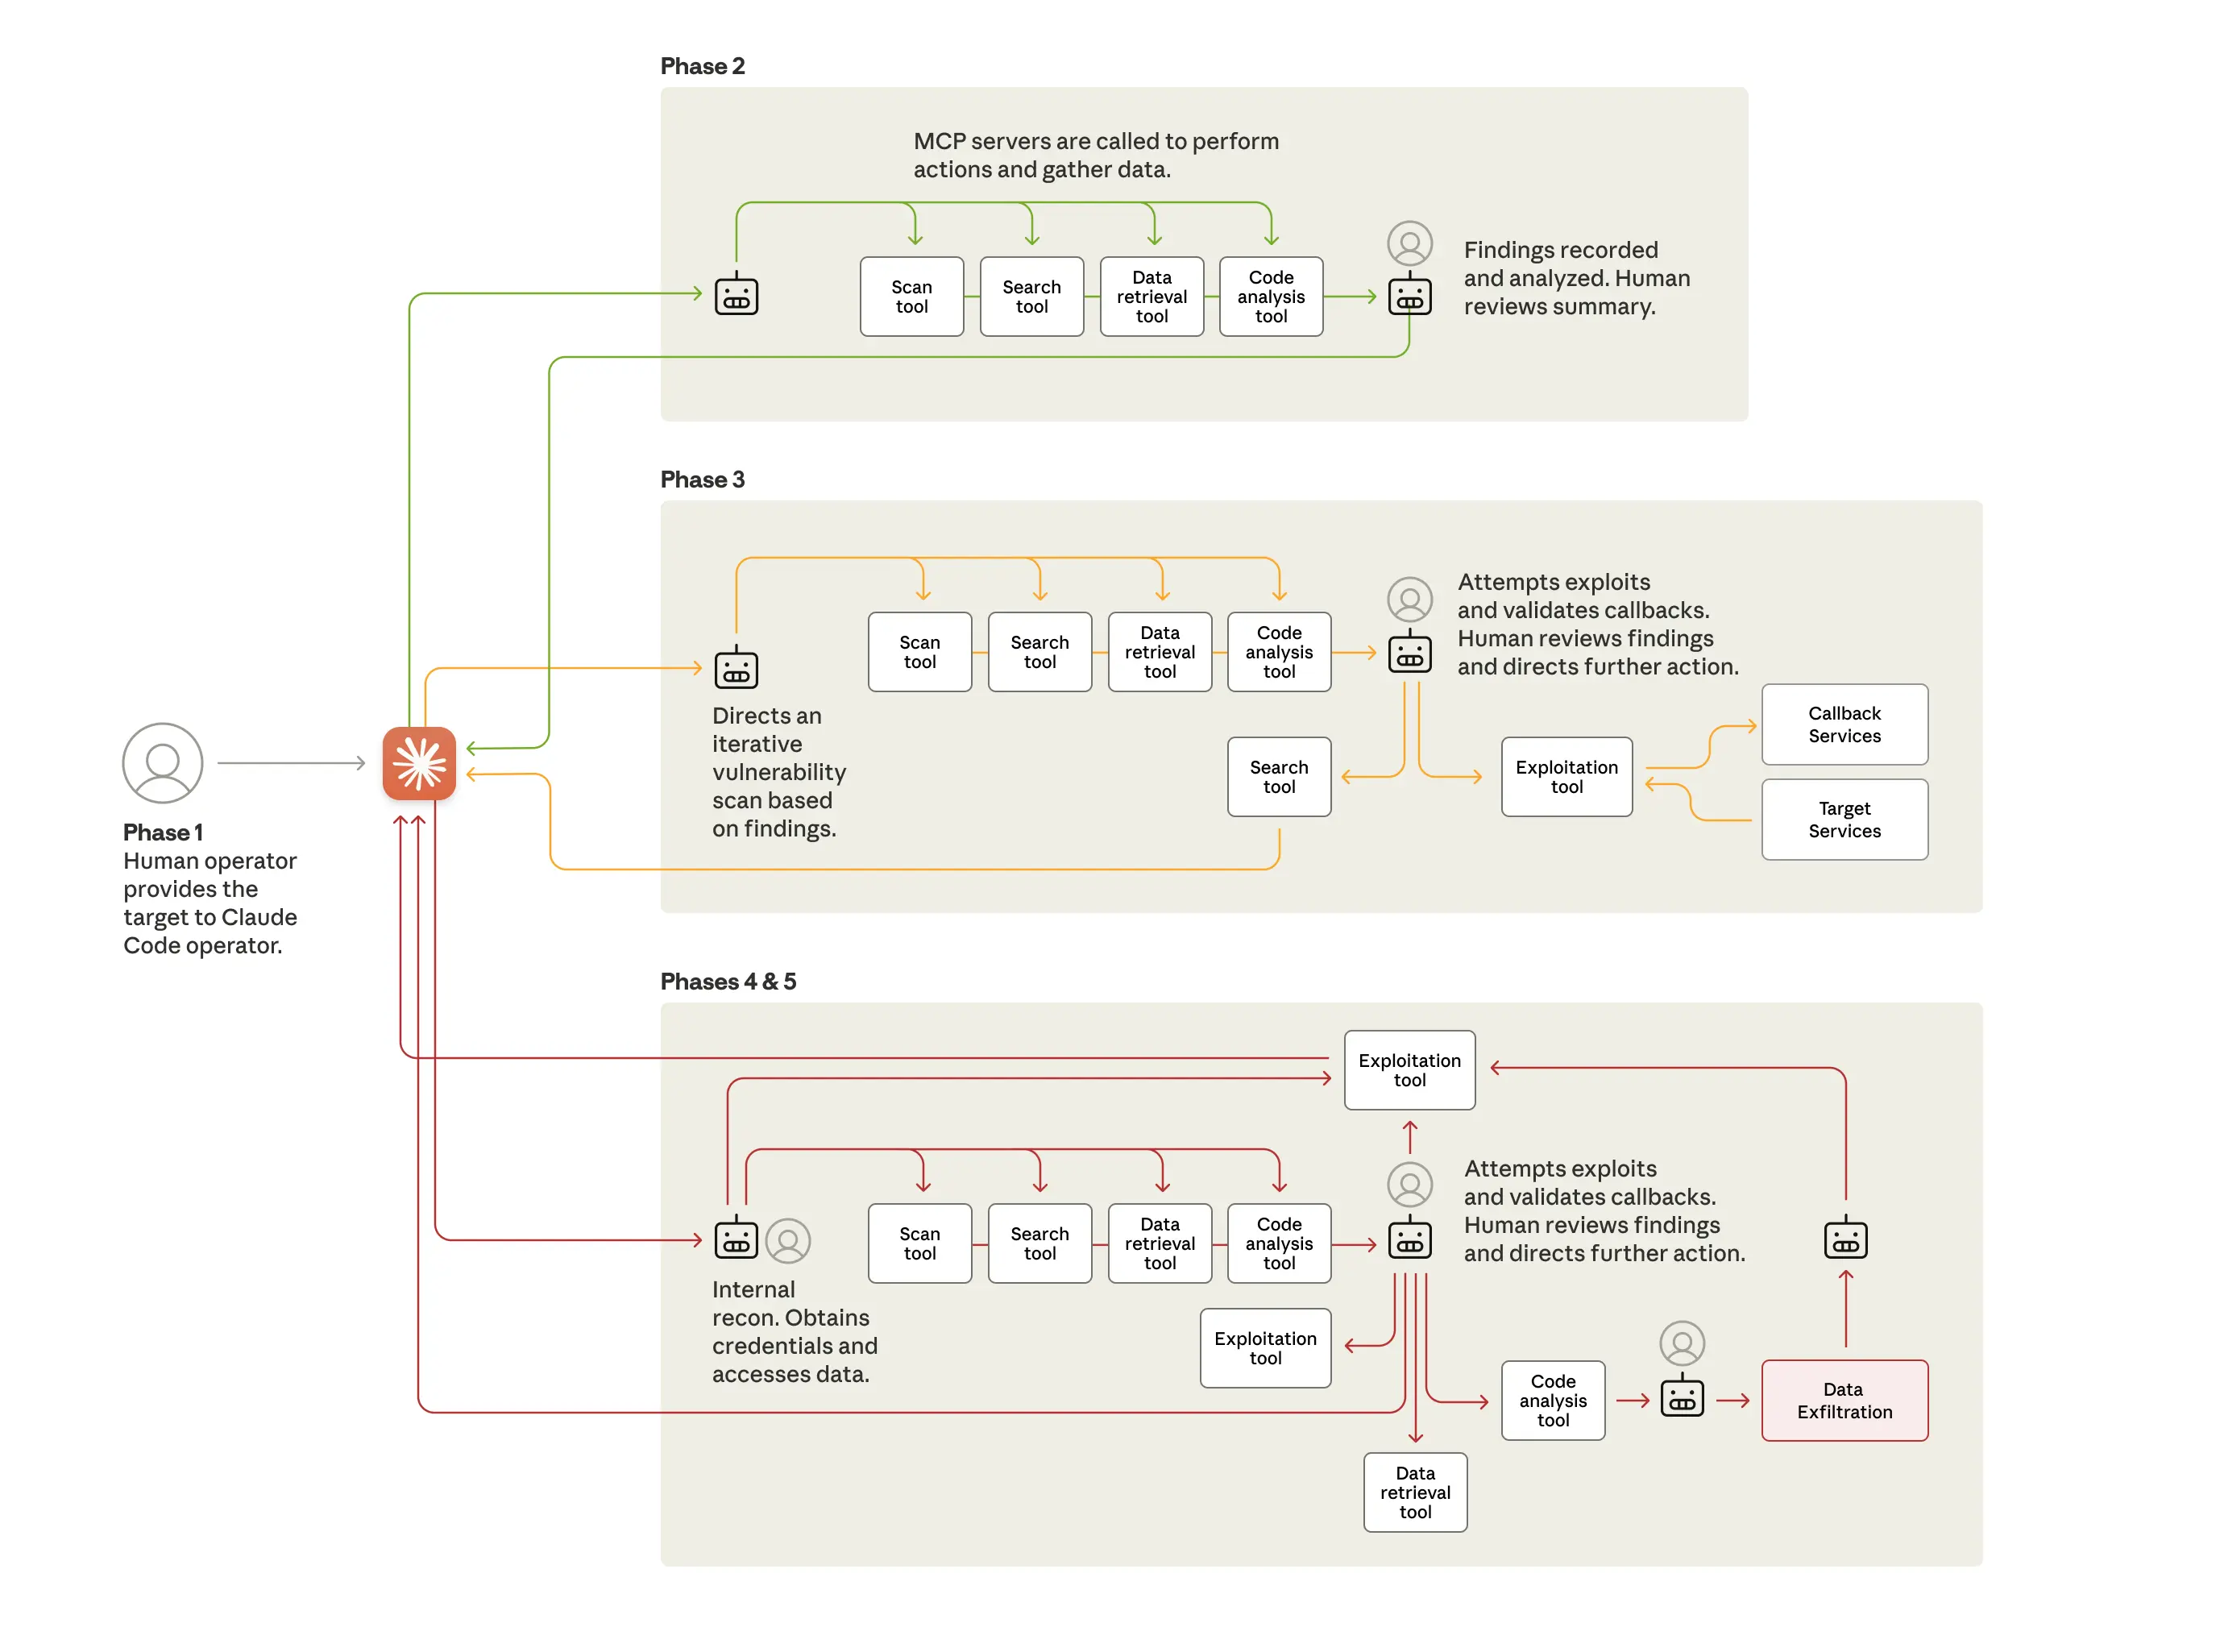
\includegraphics[width=0.9\textwidth]{claude.png}
    \caption{The lifecycle of the cyberattack, showing the transition from human-led targeting to largely AI-driven execution using various tools (often via the Model Context Protocol). At various points during the attack, the AI returns to its human operator for review and further direction~\citep{anthropic2025ai}.}
    \label{fig:claude_attack}
\end{figure}

Notably, the campaign did not depend on gradient access, white-box model knowledge, or optimized adversarial perturbations. Instead, it exploited deployment-level assumptions: that a capable model given autonomy and tools will reliably act in accordance with high-level intent. Although the AI occasionally hallucinated credentials or misclassified public data as sensitive, the overall campaign demonstrated that frontier models can materially lower the cost and scale of sophisticated cyber operations when embedded into agentic frameworks~\citep{anthropic2025ai}. This incident thus exemplifies a widening gap between prevailing academic threat models and the operational realities of adversarial ML misuse.

\subsection{Other Documented Real-World Adversarial Incidents}

The Claude case is not an isolated anomaly. Other documented incidents illustrate complementary modes of adversarial behavior in deployed ML systems. In 2025, EchoLeak, a zero-click indirect prompt injection vulnerability in Microsoft 365 Copilot, enabled the exfiltration of sensitive enterprise data through maliciously crafted documents, without requiring user interaction beyond opening a file~\citep{aim2025echoleak}. Similarly, researchers demonstrated AgentFlayer, a supply-chain prompt injection attack against ChatGPT connectors, in which poisoned documents triggered unauthorized access and data leakage across integrated enterprise tools~\citep{zenity2025agentflayer}.

Beyond prompt injection and agent misuse, black-box extraction attacks have also materialized. In 2023, researchers showed that carefully structured prompts against deployed ChatGPT models could induce verbatim leakage of training data, including personal and proprietary information, at modest cost~\citep{nasr2023scalable}. Separately, partial model extraction attacks against production language model APIs have demonstrated the feasibility of recovering proprietary model components using only query access~\citep{carlini2024stealing}. Finally, generative models have been used operationally for adversarial ends outside of ML systems themselves, most visibly in deepfake-enabled fraud, where AI-generated voice and video impersonation has led to confirmed financial losses in real organizations~\citep{guardian2024deepfake}.

These cases highlight themes that recur throughout this review: adversarial threats span technical and human factors, and real attackers often find simple exploits that circumvent defenses envisaged in academic settings. They underscore the importance of considering system integrations, content sanitization, rate limiting, and user education alongside model-centric robustness. Taken together, these incidents reveal a consistent pattern: real-world adversaries rarely operate under the assumptions most commonly studied in adversarial ML research. Instead, they exploit system integration points, automation, human trust, and economic leverage---factors that remain underrepresented in benchmark-driven evaluations. The following sections quantify the extent to which such operational considerations are reflected in contemporary adversarial ML research.

%==============================================================================
% 4. METHODOLOGY
%==============================================================================
\section{Methodology}

\subsection{Data Collection}

We conducted a systematic review of adversarial ML papers published from 2022 through 2025 in four premier security venues: ACM CCS, IEEE S\&P, NDSS, and USENIX Security. These conferences represent leading outlets for security research and frequently set research directions.

Our dataset comprises 454 papers: ACM CCS contributed 118 papers (26.0\%), IEEE S\&P 79 papers (17.4\%), NDSS 49 papers (10.8\%), and USENIX Security 208 papers (45.8\%). By publication year, there were 89 papers from 2022, 136 from 2023, 198 from 2024, and 31 from 2025 (partial year). Papers were identified through keyword searches (including ``adversarial,'' ``backdoor,'' ``poisoning,'' ``robustness'') across proceedings and digital libraries, supplemented by cross-referencing papers cited in Apruzzese et al.~\citep{apruzzese2022real}. Each candidate was manually verified to confirm primary focus on adversarial ML topics.

\begin{figure}[H]
    \centering
    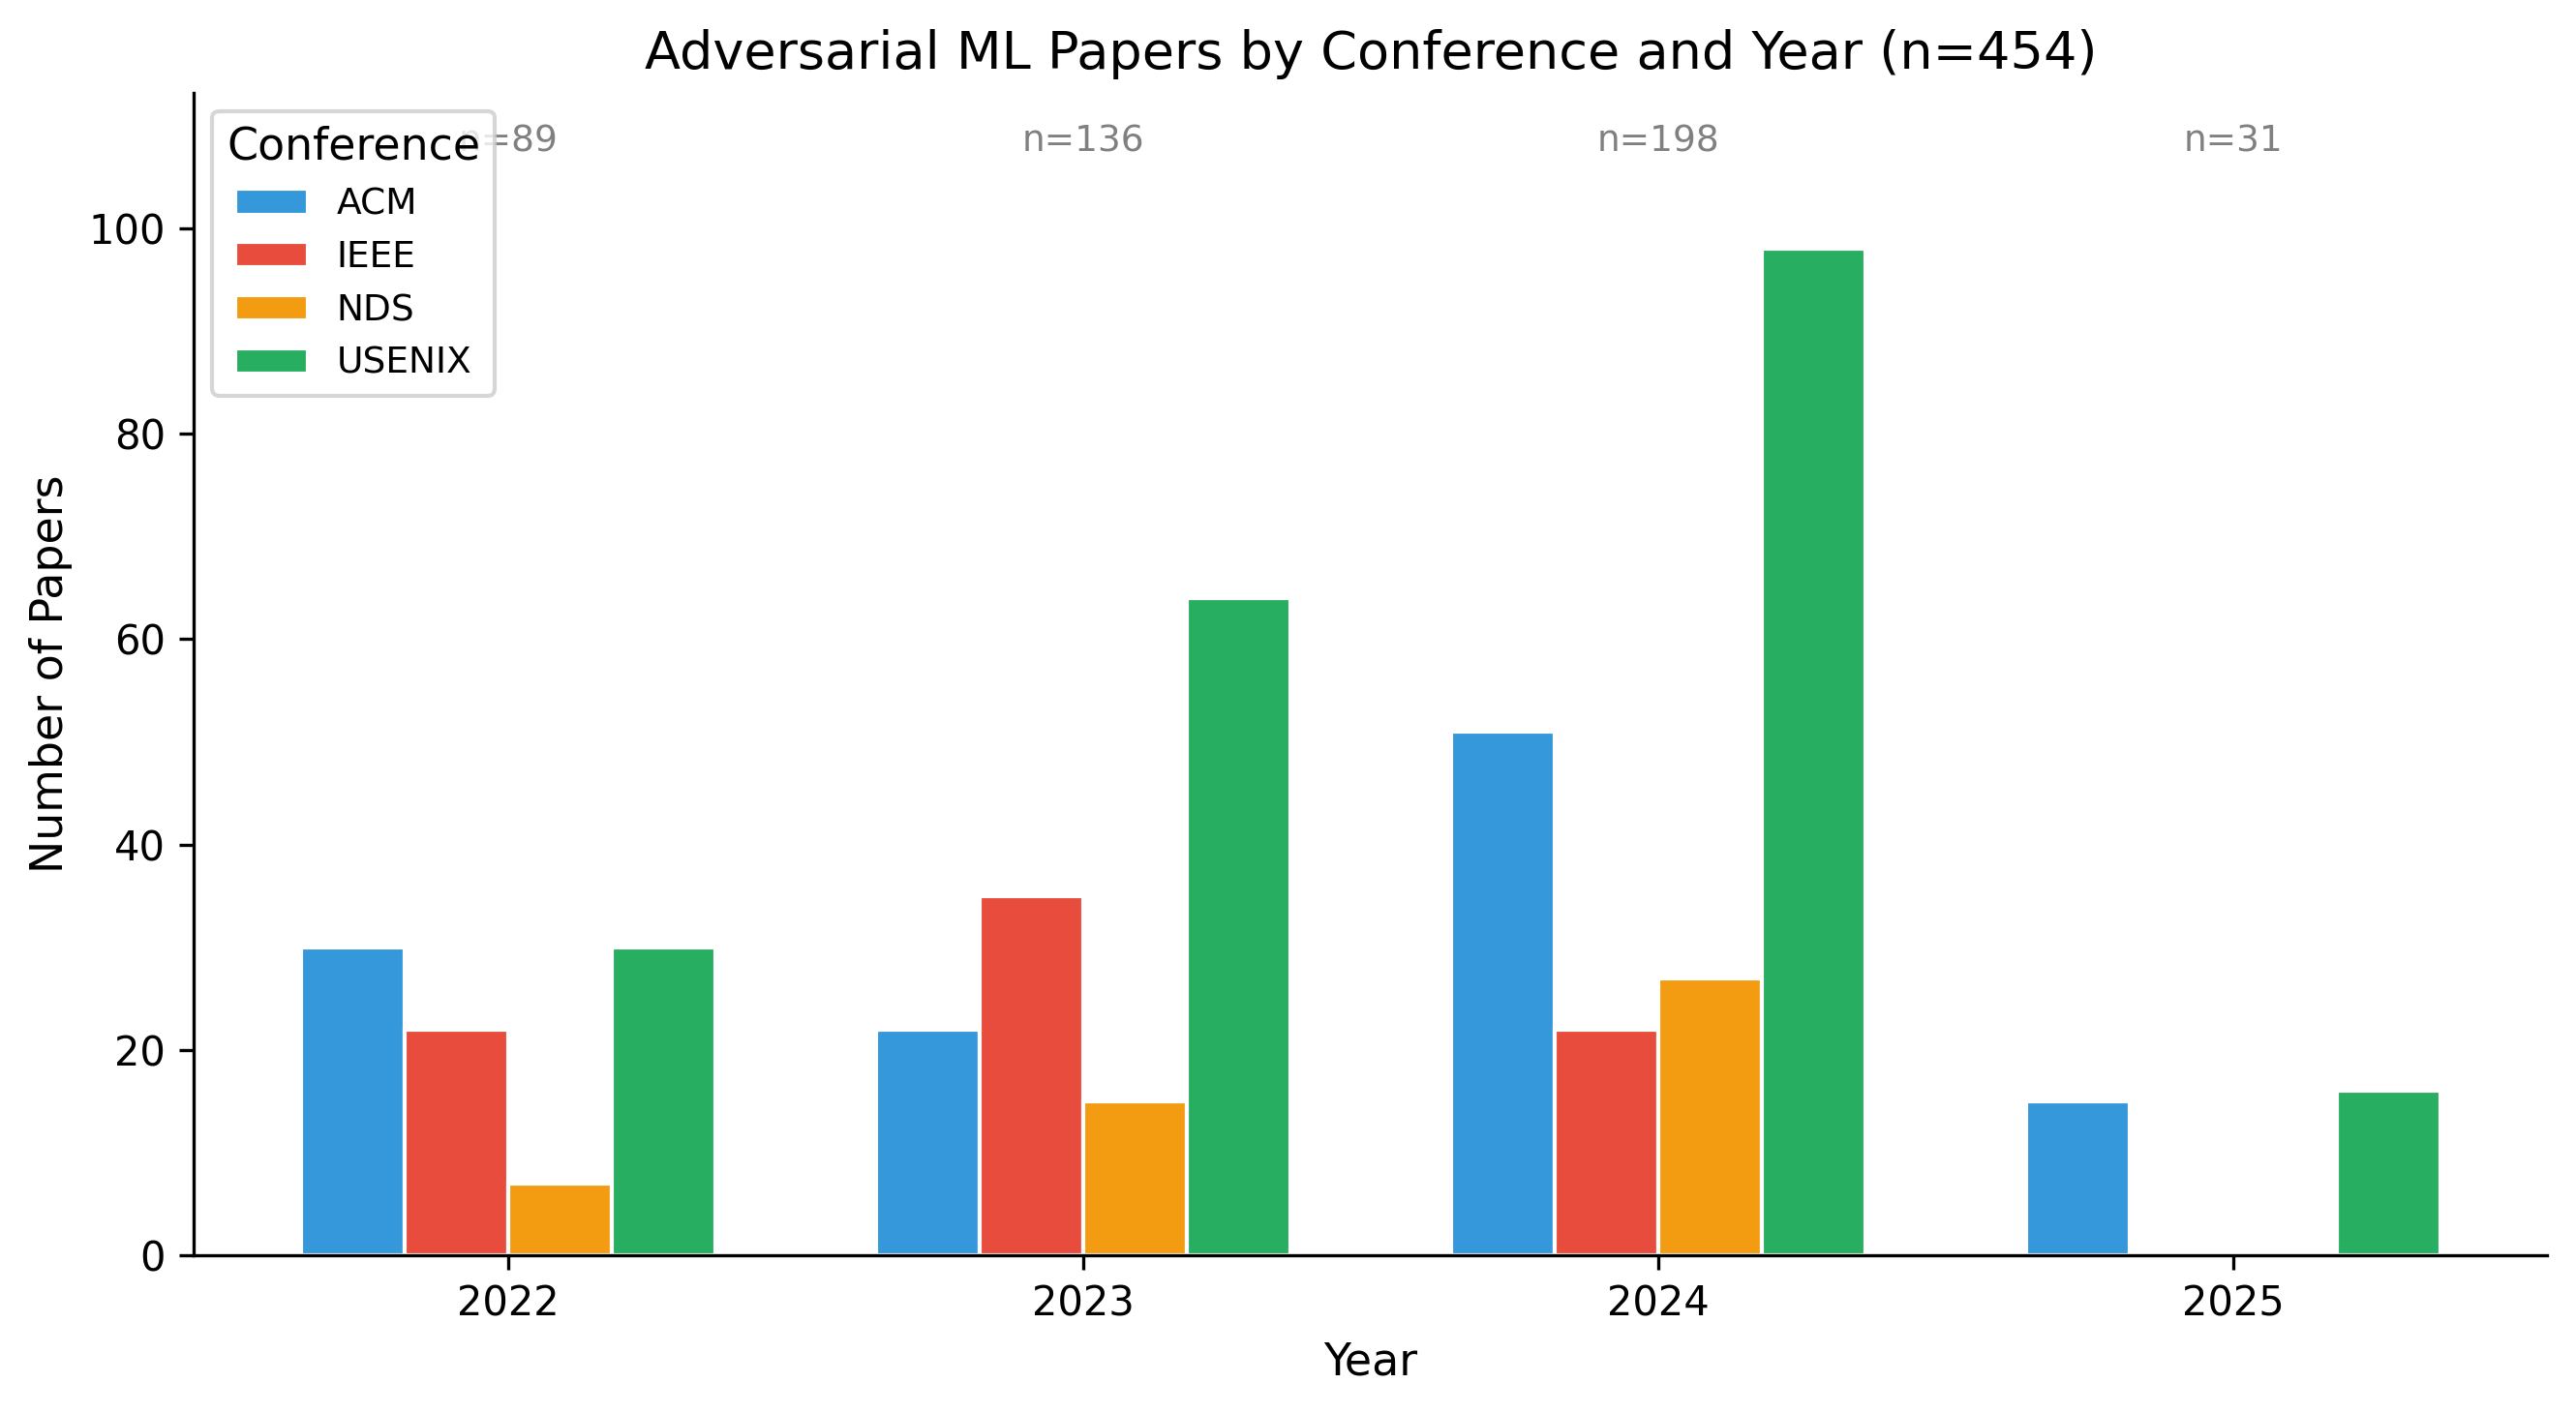
\includegraphics[width=0.9\textwidth]{fig01_dataset_overview.png}
    \caption{Dataset overview: distribution of the 454 adversarial ML papers across four security conferences from 2022 through 2025.}
    \label{fig:dataset}
\end{figure}

\subsection{Coding Framework}

Each paper was coded on dimensions adapted from Apruzzese et al.~\citep{apruzzese2022real} with additional practical considerations:

\begin{itemize}[noitemsep]
    \item \textbf{Research Focus (G1):} Attack, defense, or both.
    \item \textbf{Attack Type (G2):} Evasion, poisoning/backdoor, privacy, or multiple.
    \item \textbf{Data Domain (G4):} Images, text, audio, malware, or other.
    \item \textbf{Threat Model (T1):} White-box, black-box, or gray-box adversary knowledge.
    \item \textbf{Gradient Access (Q1):} Whether the method requires target model gradients.
    \item \textbf{Query Budget (Q2):} High ($>$1000 queries) or low budget assumption.
    \item \textbf{Real System Testing (G7):} Evaluation on deployed or production systems.
    \item \textbf{Code Release (G6):} Public availability of implementation artifacts.
    \item \textbf{Economic Consideration (G5):} Discussion of costs, incentives, or organizational factors.
\end{itemize}

Coding was performed by the authors using categorical labels and binary flags. A random 10\% subset was independently verified to ensure consistency, with ambiguous cases resolved through discussion.

\subsection{Gap Score}

To quantify divergence from practical conditions, we computed a ``Gap Score'' based on six factors:

\begin{enumerate}[noitemsep,label=(\arabic*)]
    \item Assumes white-box adversary.
    \item Requires gradient computation from target model.
    \item Assumes high query budget ($>$1000 queries).
    \item Requires substantial computational resources.
    \item Lacks real system or deployment testing.
    \item Omits economic or organizational factors.
\end{enumerate}

Each paper received a score from 0 (aligned with practical constraints) to 6 (entirely idealized assumptions). While this heuristic assigns equal weight to factors that may differ in importance, it provides a tractable measure of practical orientation for comparative analysis.

%==============================================================================
% 5. QUANTITATIVE FINDINGS
%==============================================================================
\section{Quantitative Findings}

\begin{figure}[H]
    \centering
    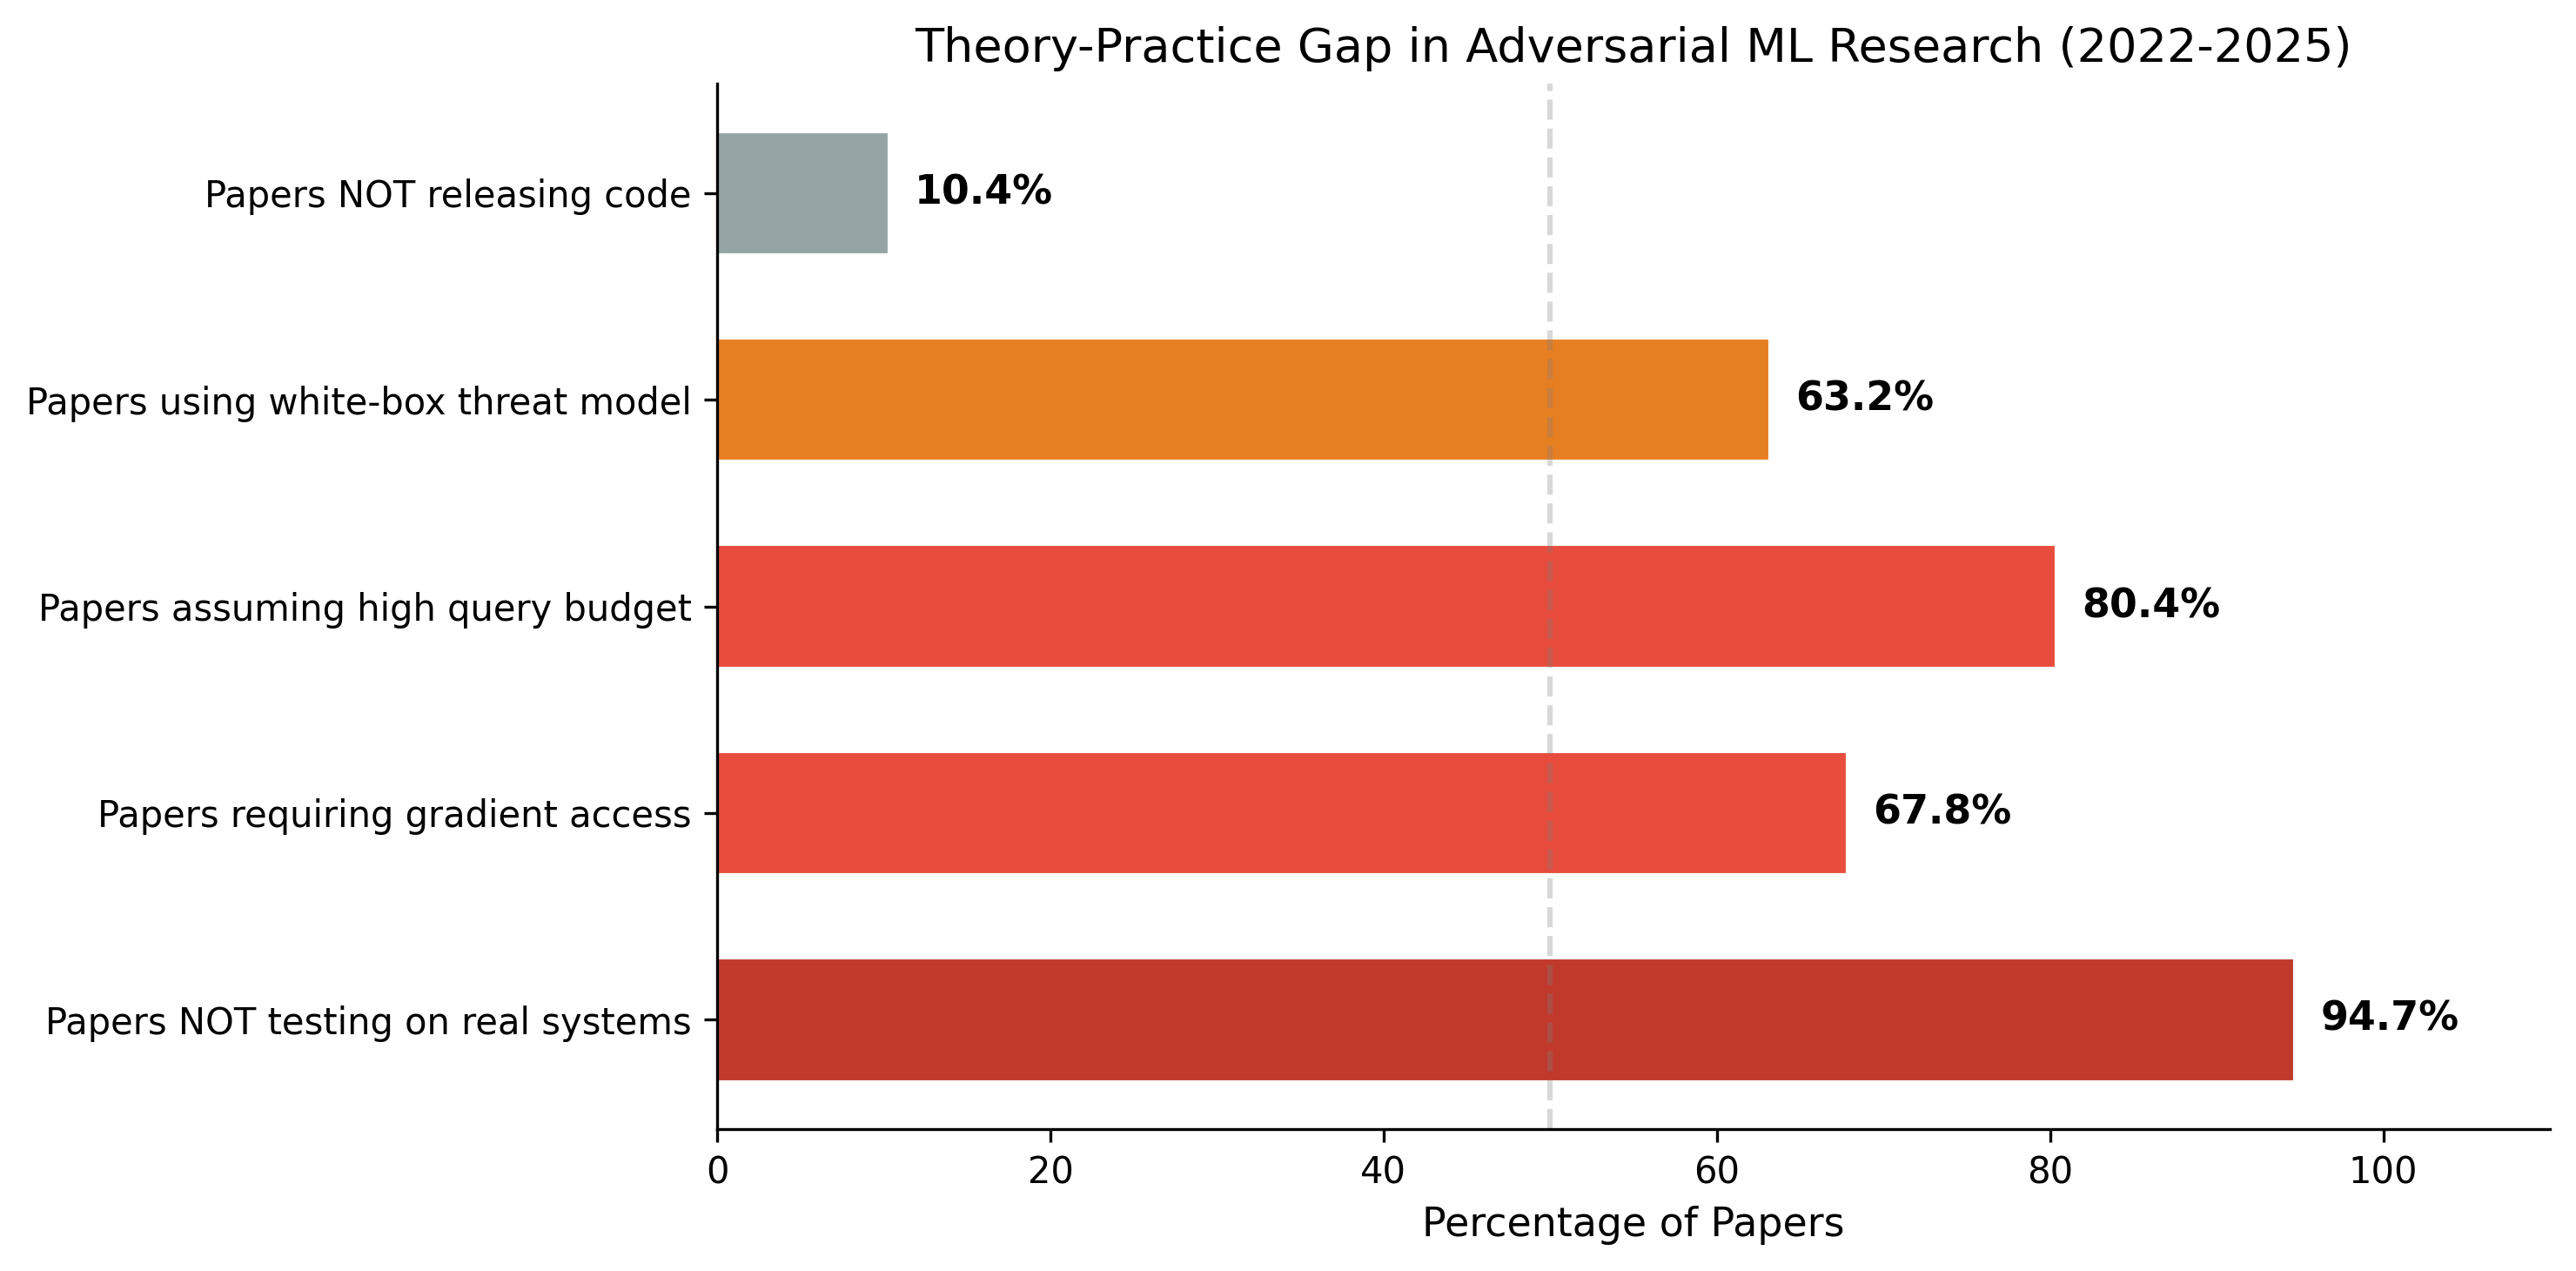
\includegraphics[width=0.9\textwidth]{fig02_theory_practice_gap.png}
    \caption{Key indicators of the theory-practice gap: percentage of papers exhibiting each characteristic.}
    \label{fig:gap_overview}
\end{figure}

Our analysis identifies several dimensions where current research practices diverge from deployment realities.

\subsection{Real-World Evaluation}

Evaluation on production systems remains rare. Only \textbf{5.3\%} of papers (24 of 454) included experiments on operational systems or realistic deployment settings; the remainder relied on offline datasets, simulated environments, or research prototypes.

\begin{figure}[H]
    \centering
    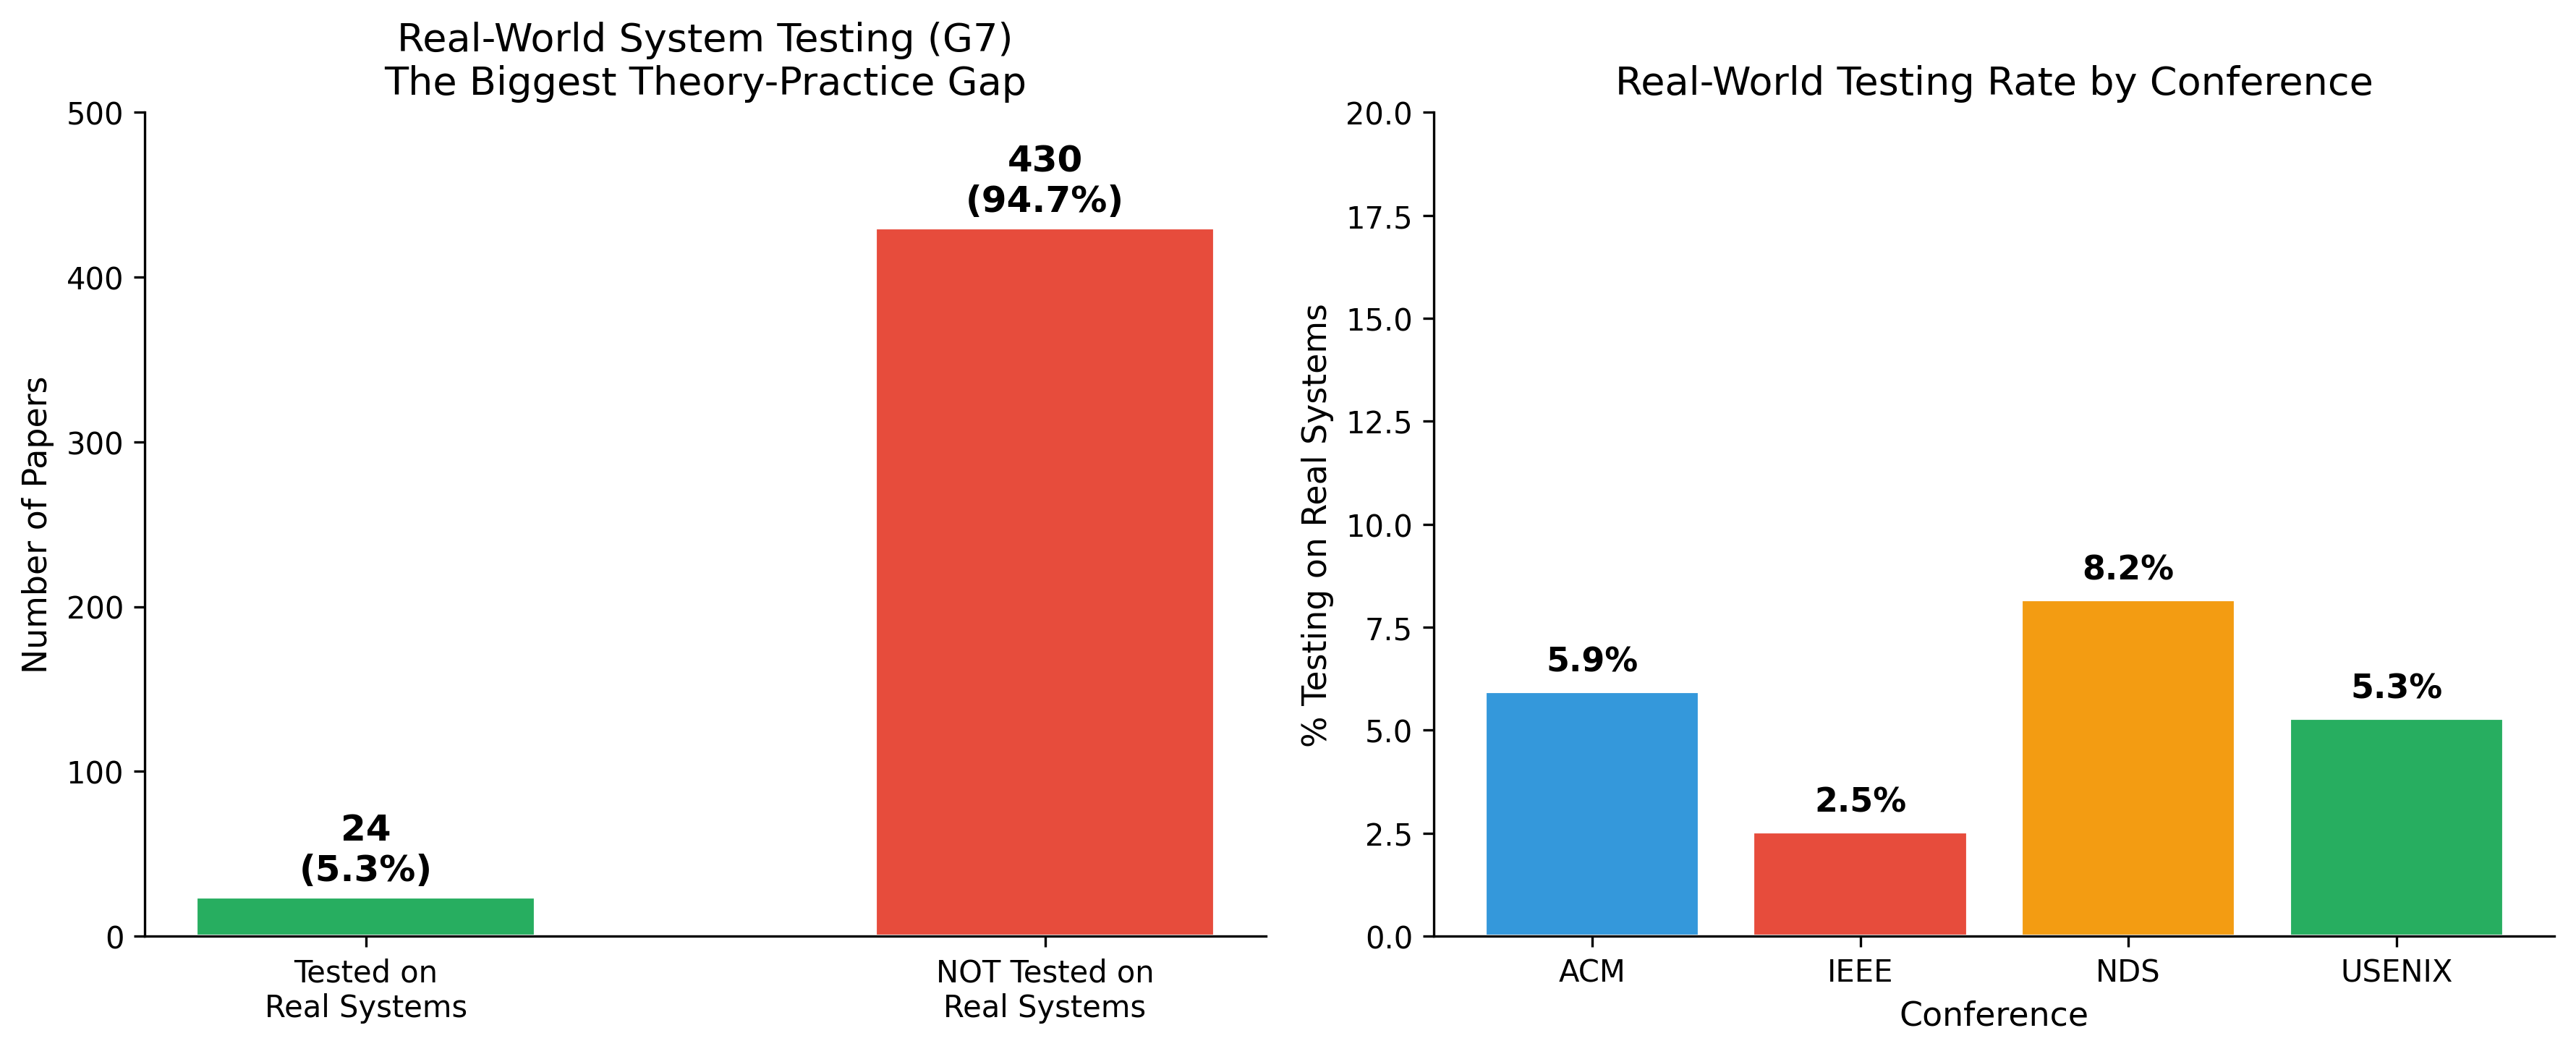
\includegraphics[width=0.9\textwidth]{fig05_real_world_testing.png}
    \caption{Rate of real-world testing: only 5.3\% of papers evaluated on deployed systems.}
    \label{fig:real_world}
\end{figure}

Deployment introduces pipeline effects, operational constraints, and monitoring absent from controlled benchmarks. The papers attempting real-world testing often revealed gaps that laboratory evaluations miss. Nayan et al.~\citep{nayan2024sok}, systematizing model extraction attacks on deployed ML APIs, found many academic attacks difficult to reproduce on actual services, with substantially degraded performance compared to constrained settings. Layton et al.~\citep{layton2024sok} observed similar patterns for deepfake detection algorithms when evaluated on real-world distributions.

Duan et al.~\citep{duan2022perception} provide a notable example: they crafted adversarial audio to evade YouTube's content identification system, accounting for platform-specific audio compression and matching algorithms.

\subsection{Reliance on Gradients}

We found that \textbf{67.8\%} of papers require gradient information from target models, either explicitly or implicitly.

\begin{figure}[H]
    \centering
    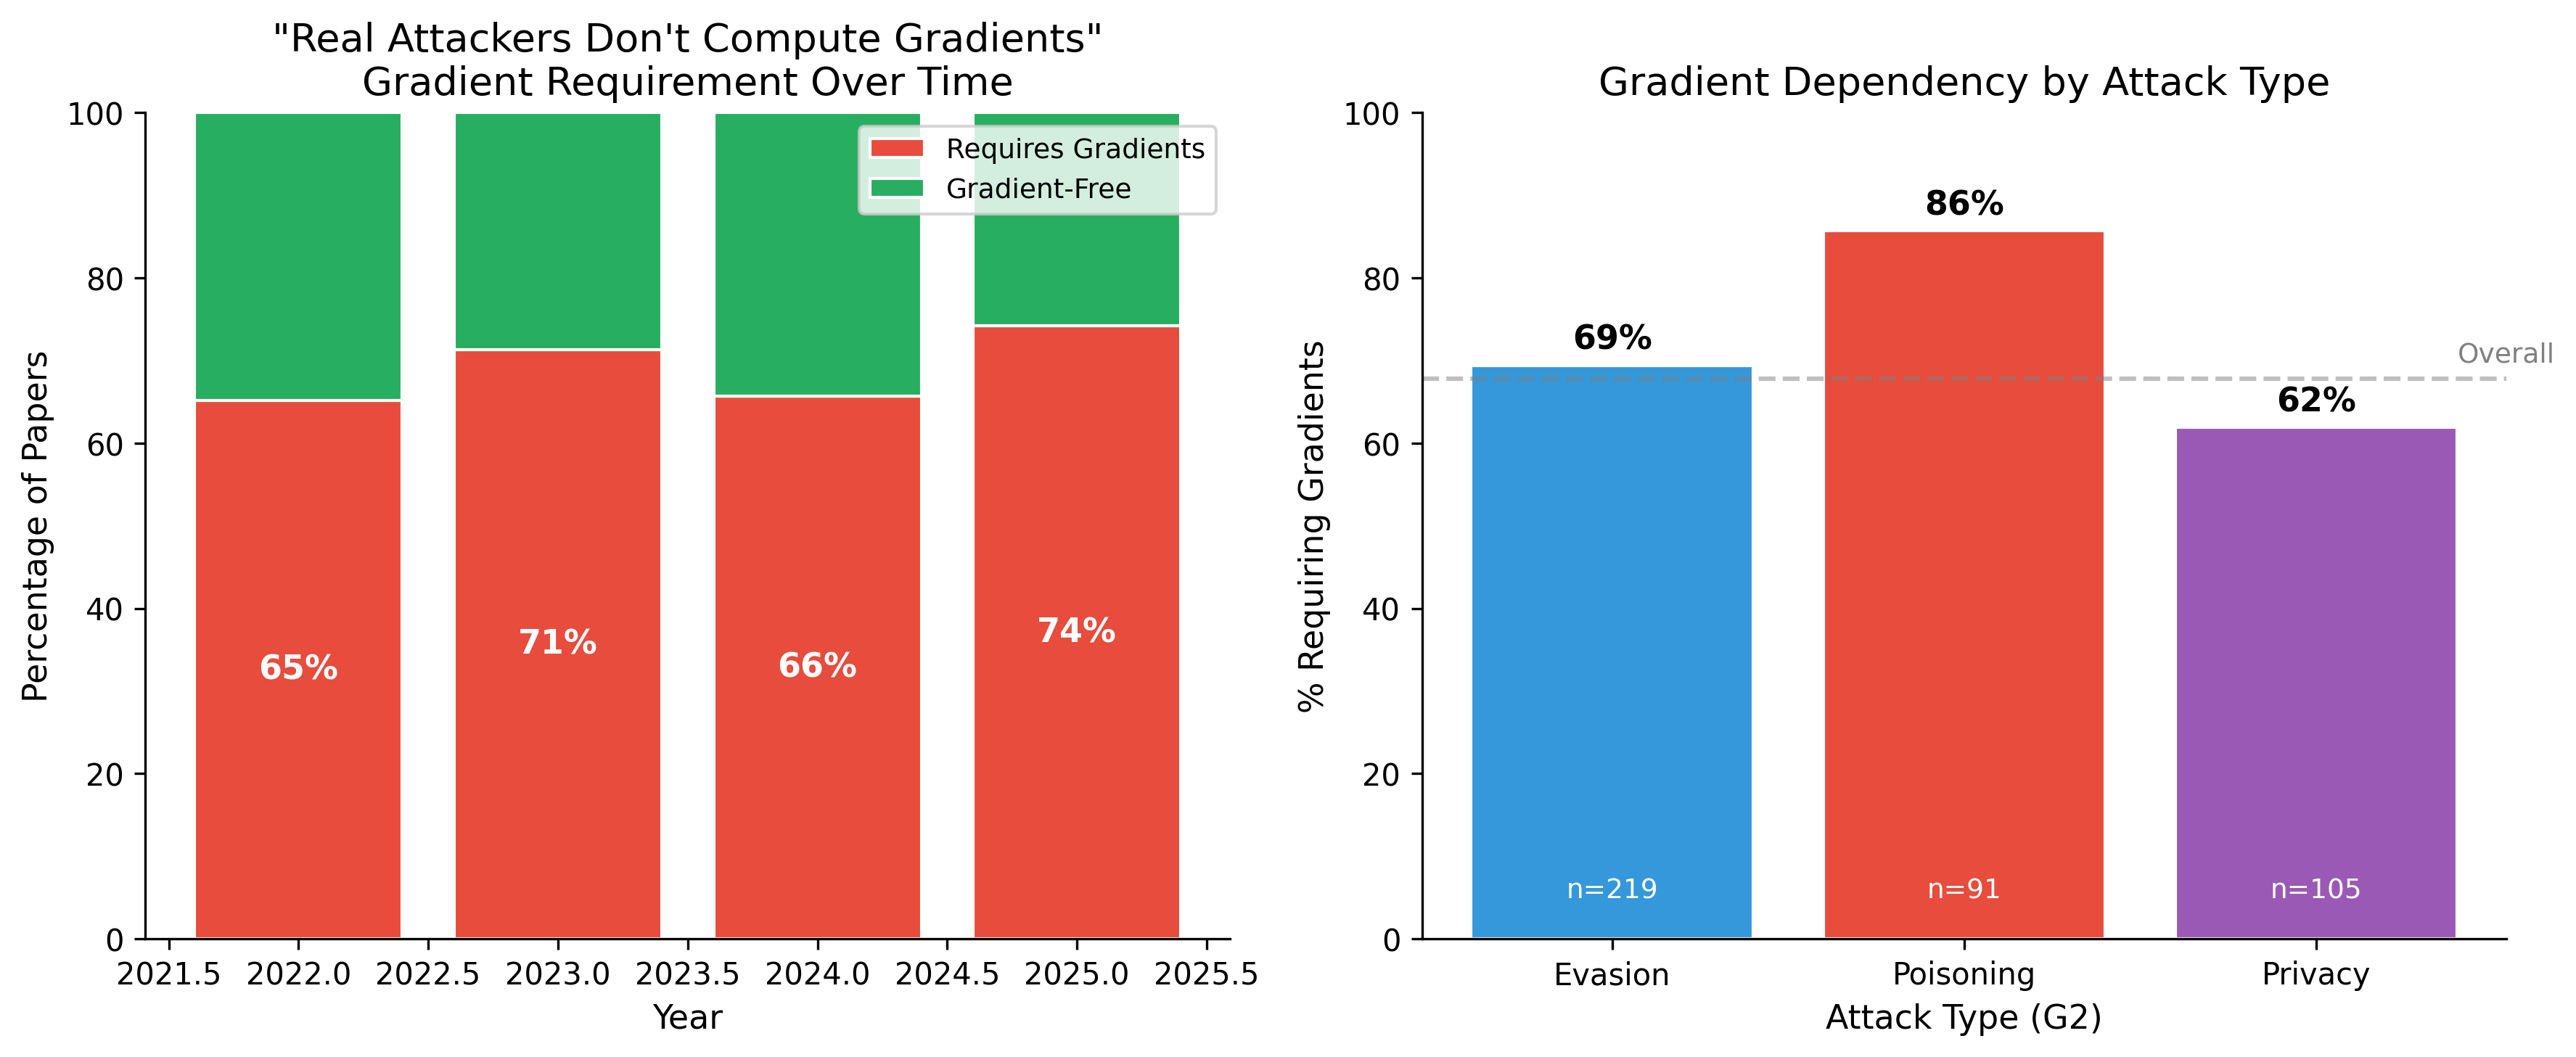
\includegraphics[width=0.9\textwidth]{fig04_gradient_dependency.png}
    \caption{Gradient dependency: 67.8\% of papers required gradient access. The proportion changed only modestly from 2022 (68.2\%) to early 2025 (65.9\%).}
    \label{fig:gradient}
\end{figure}

This persistence is notable given the critique that ``real attackers don't compute gradients''~\citep{apruzzese2022real}. Some recent work has embraced gradient-free approaches. Eykholt et al.~\citep{eykholt2023uret} developed URET, evaluating robustness through domain-specific transformations without direct gradient access. In the LLM domain, numerous jailbreak attacks operate without gradients, using only natural language interaction~\citep{liu2024jailbreaking, yu2024jailbreak}.

\subsection{Threat Model Assumptions}

We found that \textbf{63.2\%} of papers assume white-box adversaries with complete model knowledge. Only 34.1\% consider black-box scenarios, and 2.6\% explicitly explore gray-box settings.

\begin{figure}[H]
    \centering
    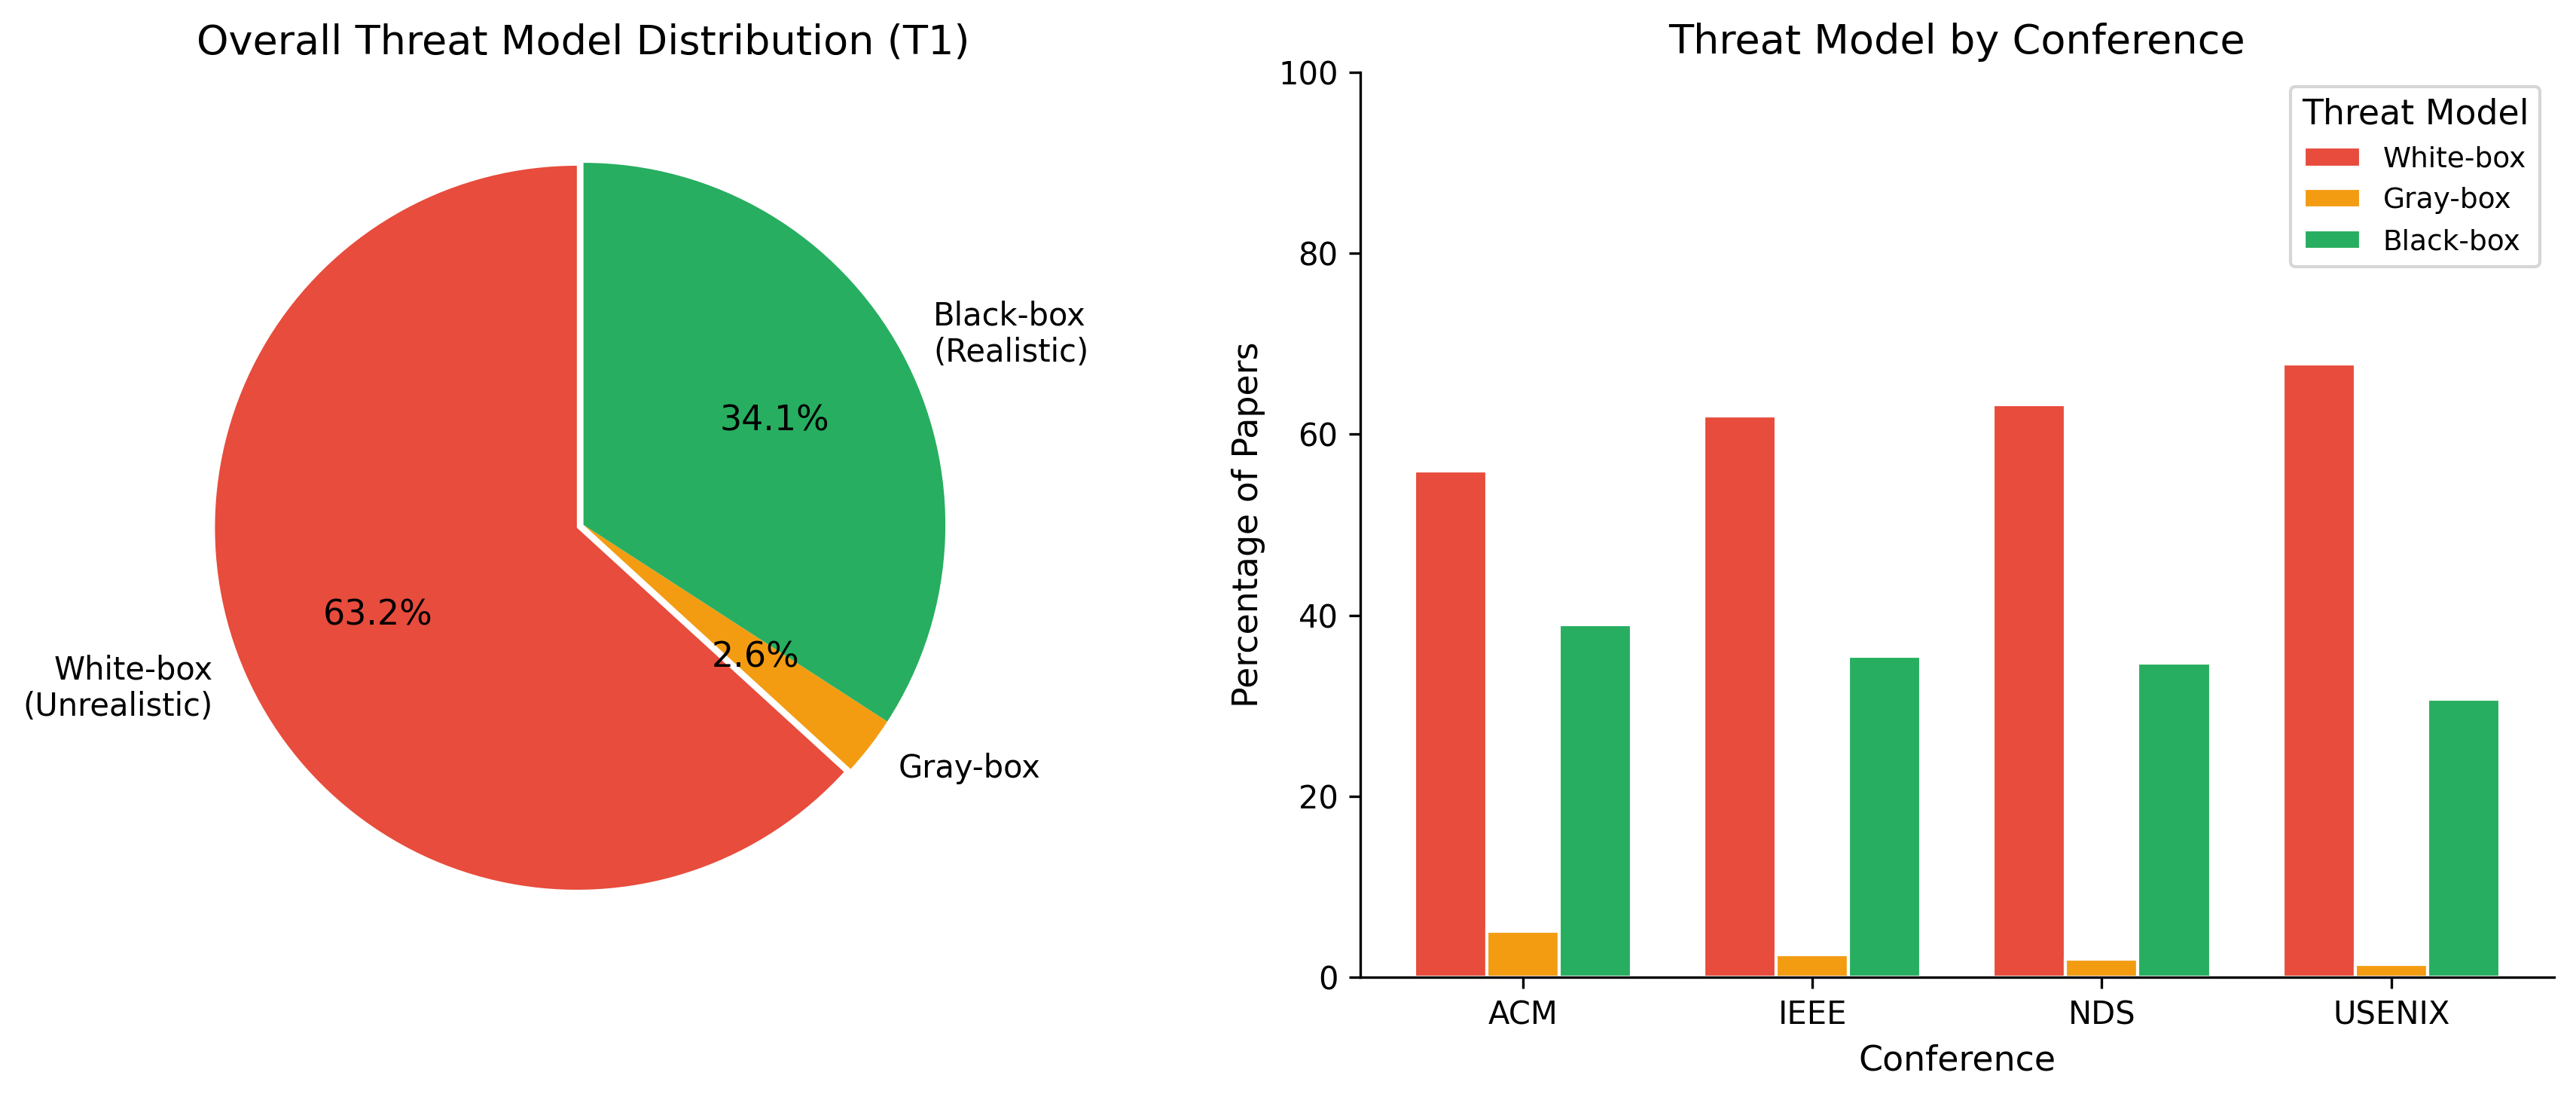
\includegraphics[width=0.9\textwidth]{fig03_threat_model.png}
    \caption{Threat model assumptions: white-box scenarios dominate at 63.2\%.}
    \label{fig:threat_model}
\end{figure}

This distribution contrasts with deployment realities where attackers rarely possess internal model access. The prevalence of white-box assumptions reflects both the technical convenience of gradient-based methods and the convention of evaluating against worst-case adversaries.

\subsection{Query Budget and Efficiency}

Among papers involving model queries, \textbf{80.4\%} assume high query budgets exceeding 1000 queries. In practice, query rates are constrained by cost, rate limiting, and anomaly detection.

\begin{figure}[H]
    \centering
    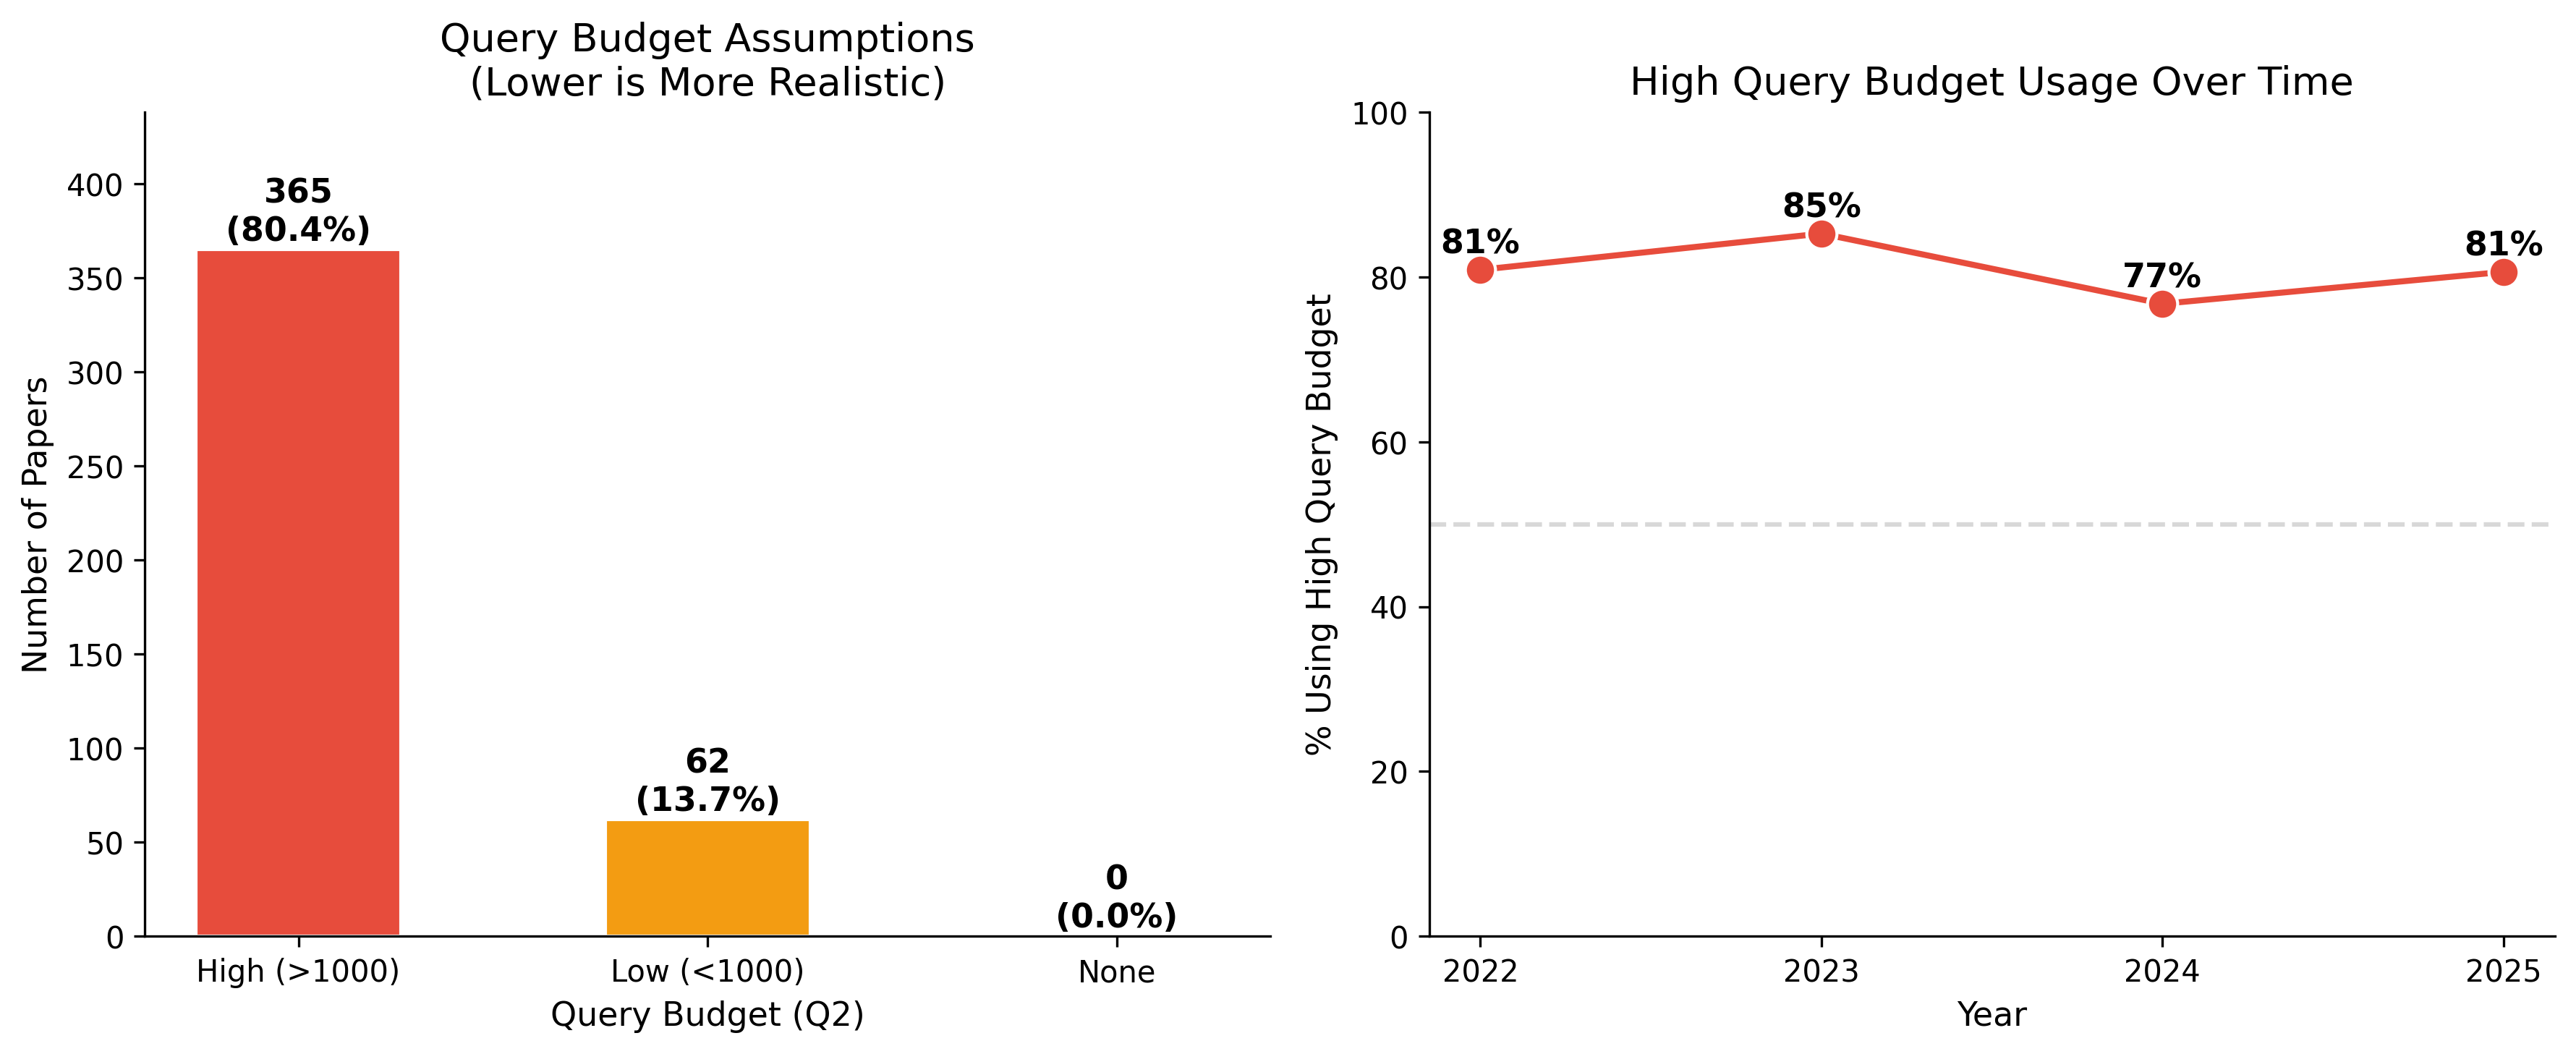
\includegraphics[width=0.9\textwidth]{fig06_query_budget.png}
    \caption{Assumed query budgets: over 80\% of relevant papers assumed high budgets ($>$1000 queries).}
    \label{fig:query}
\end{figure}

Notable exceptions demonstrate query-efficient alternatives. Tao et al.~\citep{tao2023hardbeat} proposed HARDBEAT, achieving high attack success with few queries under hard-label constraints. Wan et al.~\citep{wan2024bounceattack} developed BounceAttack, a decision-based approach requiring minimal queries.

\subsection{Dominant Data Domains}

Approximately \textbf{65\%} of papers focus on image-based tasks, with text (11\%), audio (7\%), malware (6\%), and other domains (12\%) comprising the remainder.

\begin{figure}[H]
    \centering
    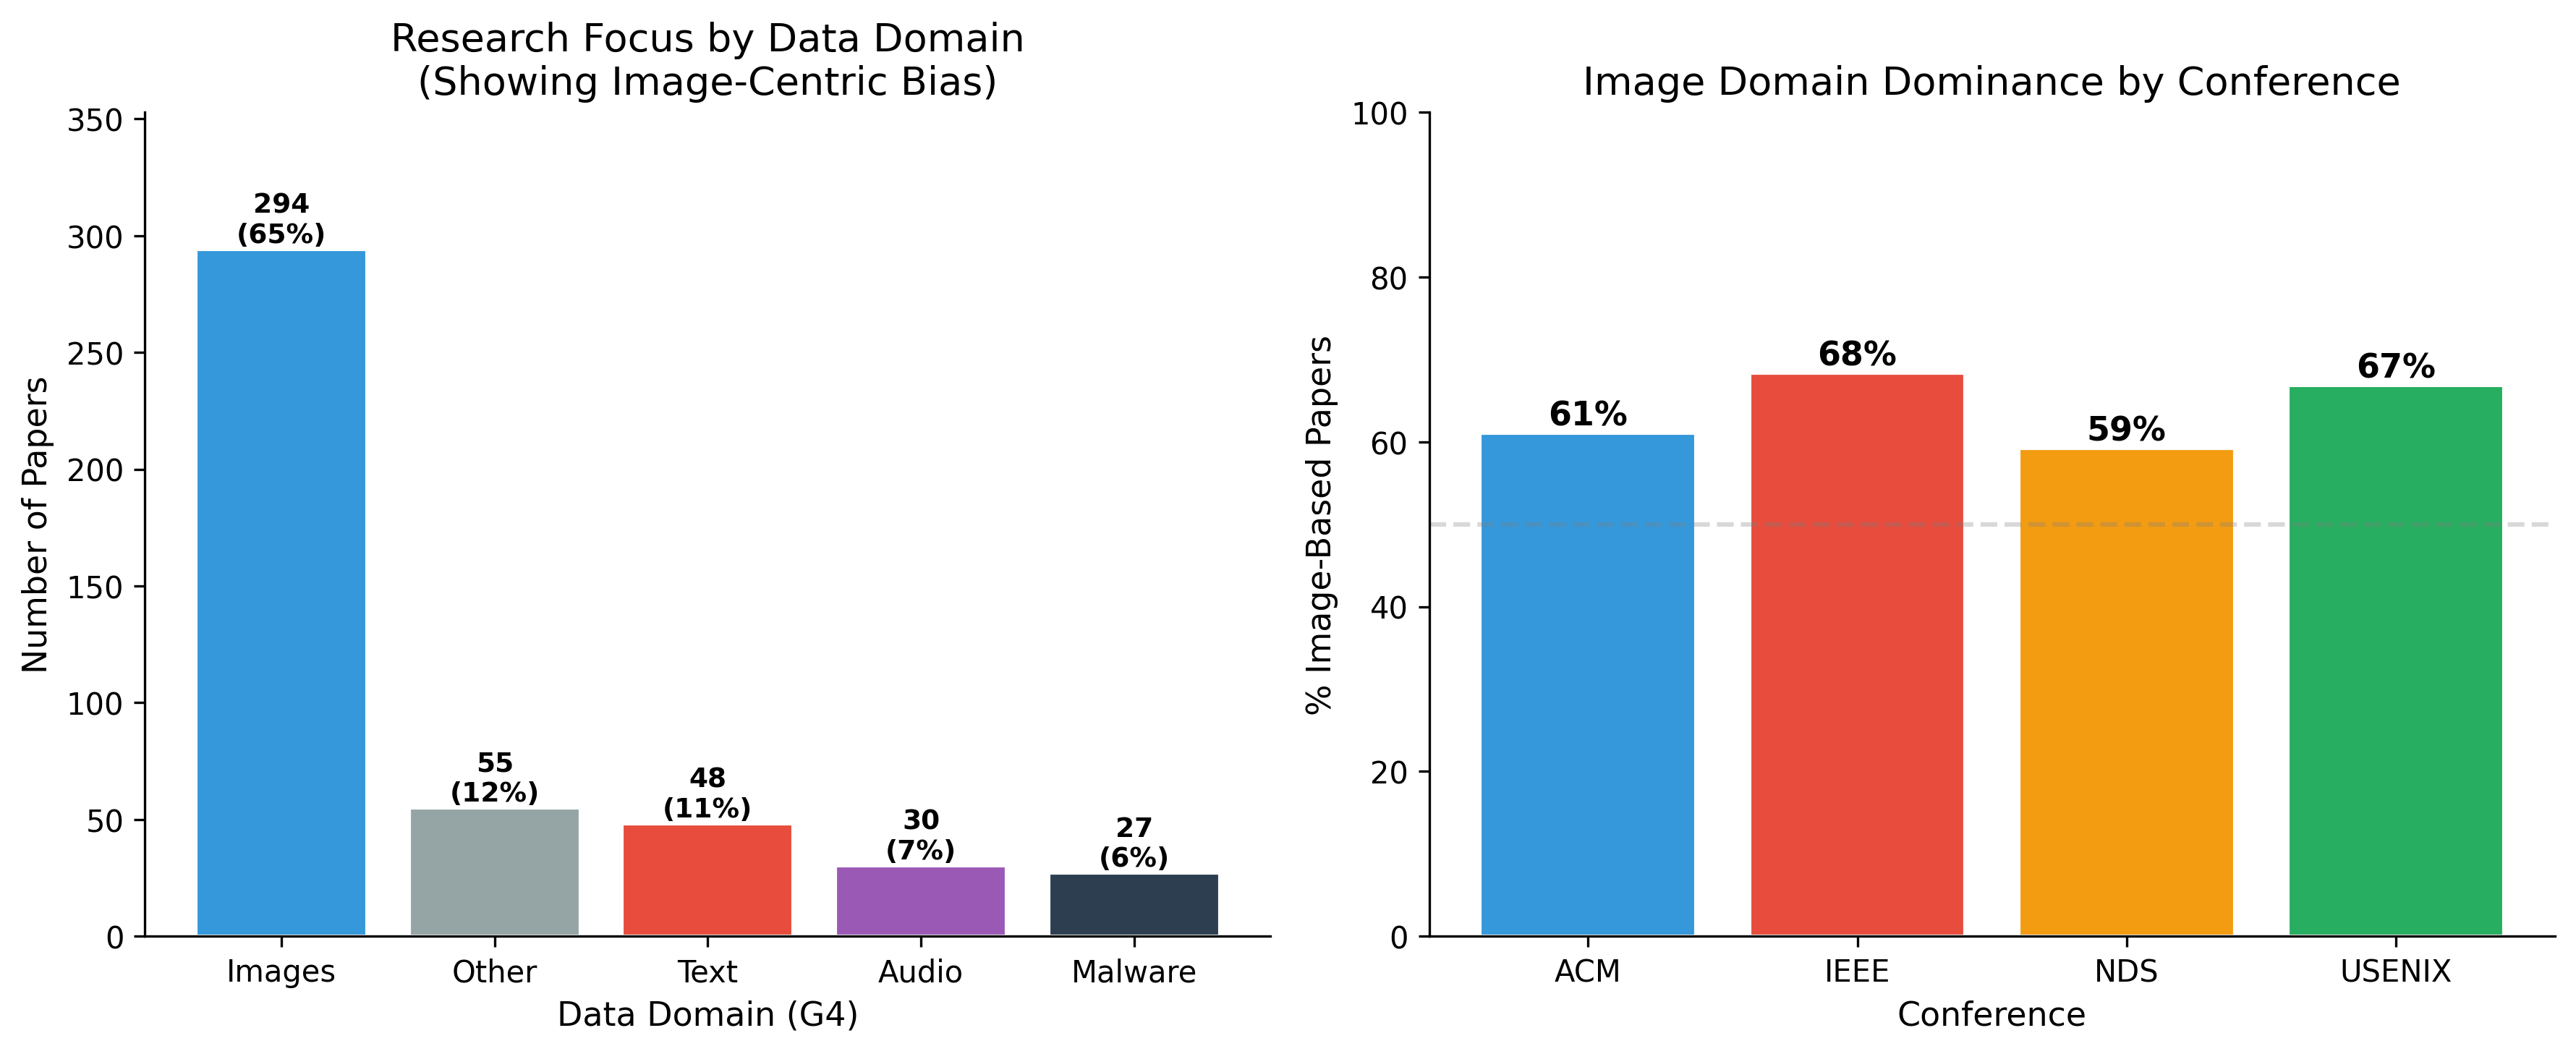
\includegraphics[width=0.9\textwidth]{fig08_data_domains.png}
    \caption{Data domains: image-focused research dominates at 65\%.}
    \label{fig:domains}
\end{figure}

This concentration reflects the historical development of adversarial ML around computer vision benchmarks. However, assumptions suitable for images may not transfer to other domains. Kireev et al.~\citep{kireev2023cost} demonstrated that in financial applications, cost-based perturbation metrics may be more meaningful than pixel norms.

\subsection{Reproducibility and Code Release}

\textbf{89.6\%} of papers provided public code or indicated intent to release artifacts. While commendable for reproducibility, research code often requires substantial adaptation for production deployment.

\subsection{Gap Score Distribution}

The average Gap Score was \textbf{3.17}, with most papers scoring 3--4. Only approximately 10.5\% scored 0 or 1, indicating close alignment with deployment constraints.

\begin{figure}[H]
    \centering
    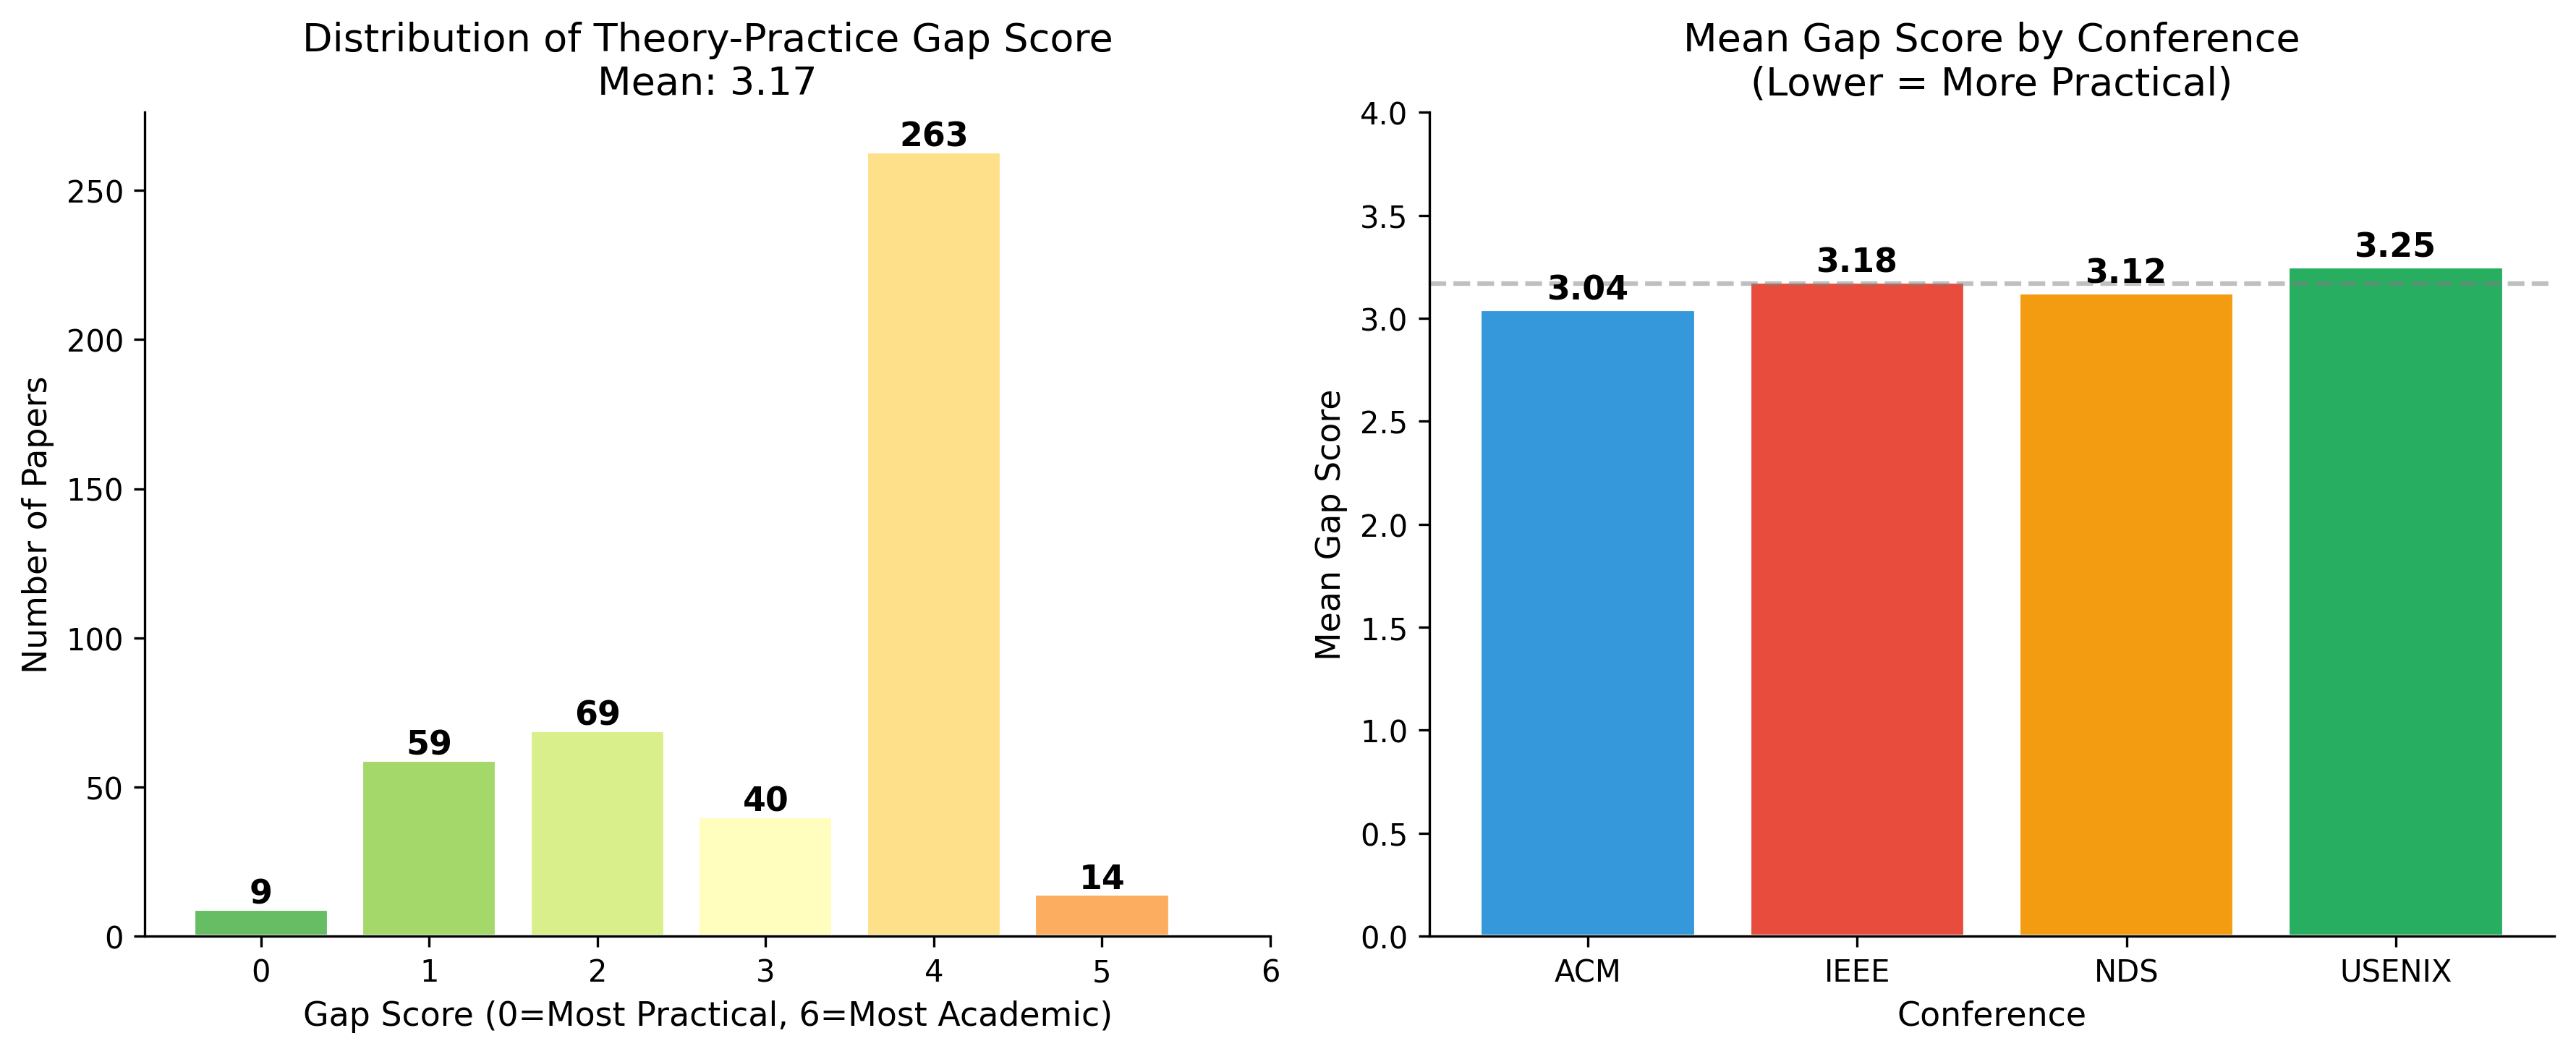
\includegraphics[width=0.9\textwidth]{fig12_gap_score.png}
    \caption{Distribution of Gap Scores: the typical paper incorporates about half of the idealized assumptions we tracked.}
    \label{fig:gap_score}
\end{figure}

Cross-venue comparison revealed similar averages: CCS approximately 3.04, NDSS approximately 3.12, S\&P approximately 3.18, and USENIX approximately 3.25.

%==============================================================================
% 6. QUALITATIVE AND THEMATIC FINDINGS
%==============================================================================
\section{Qualitative and Thematic Findings}

\begin{figure}[H]
    \centering
    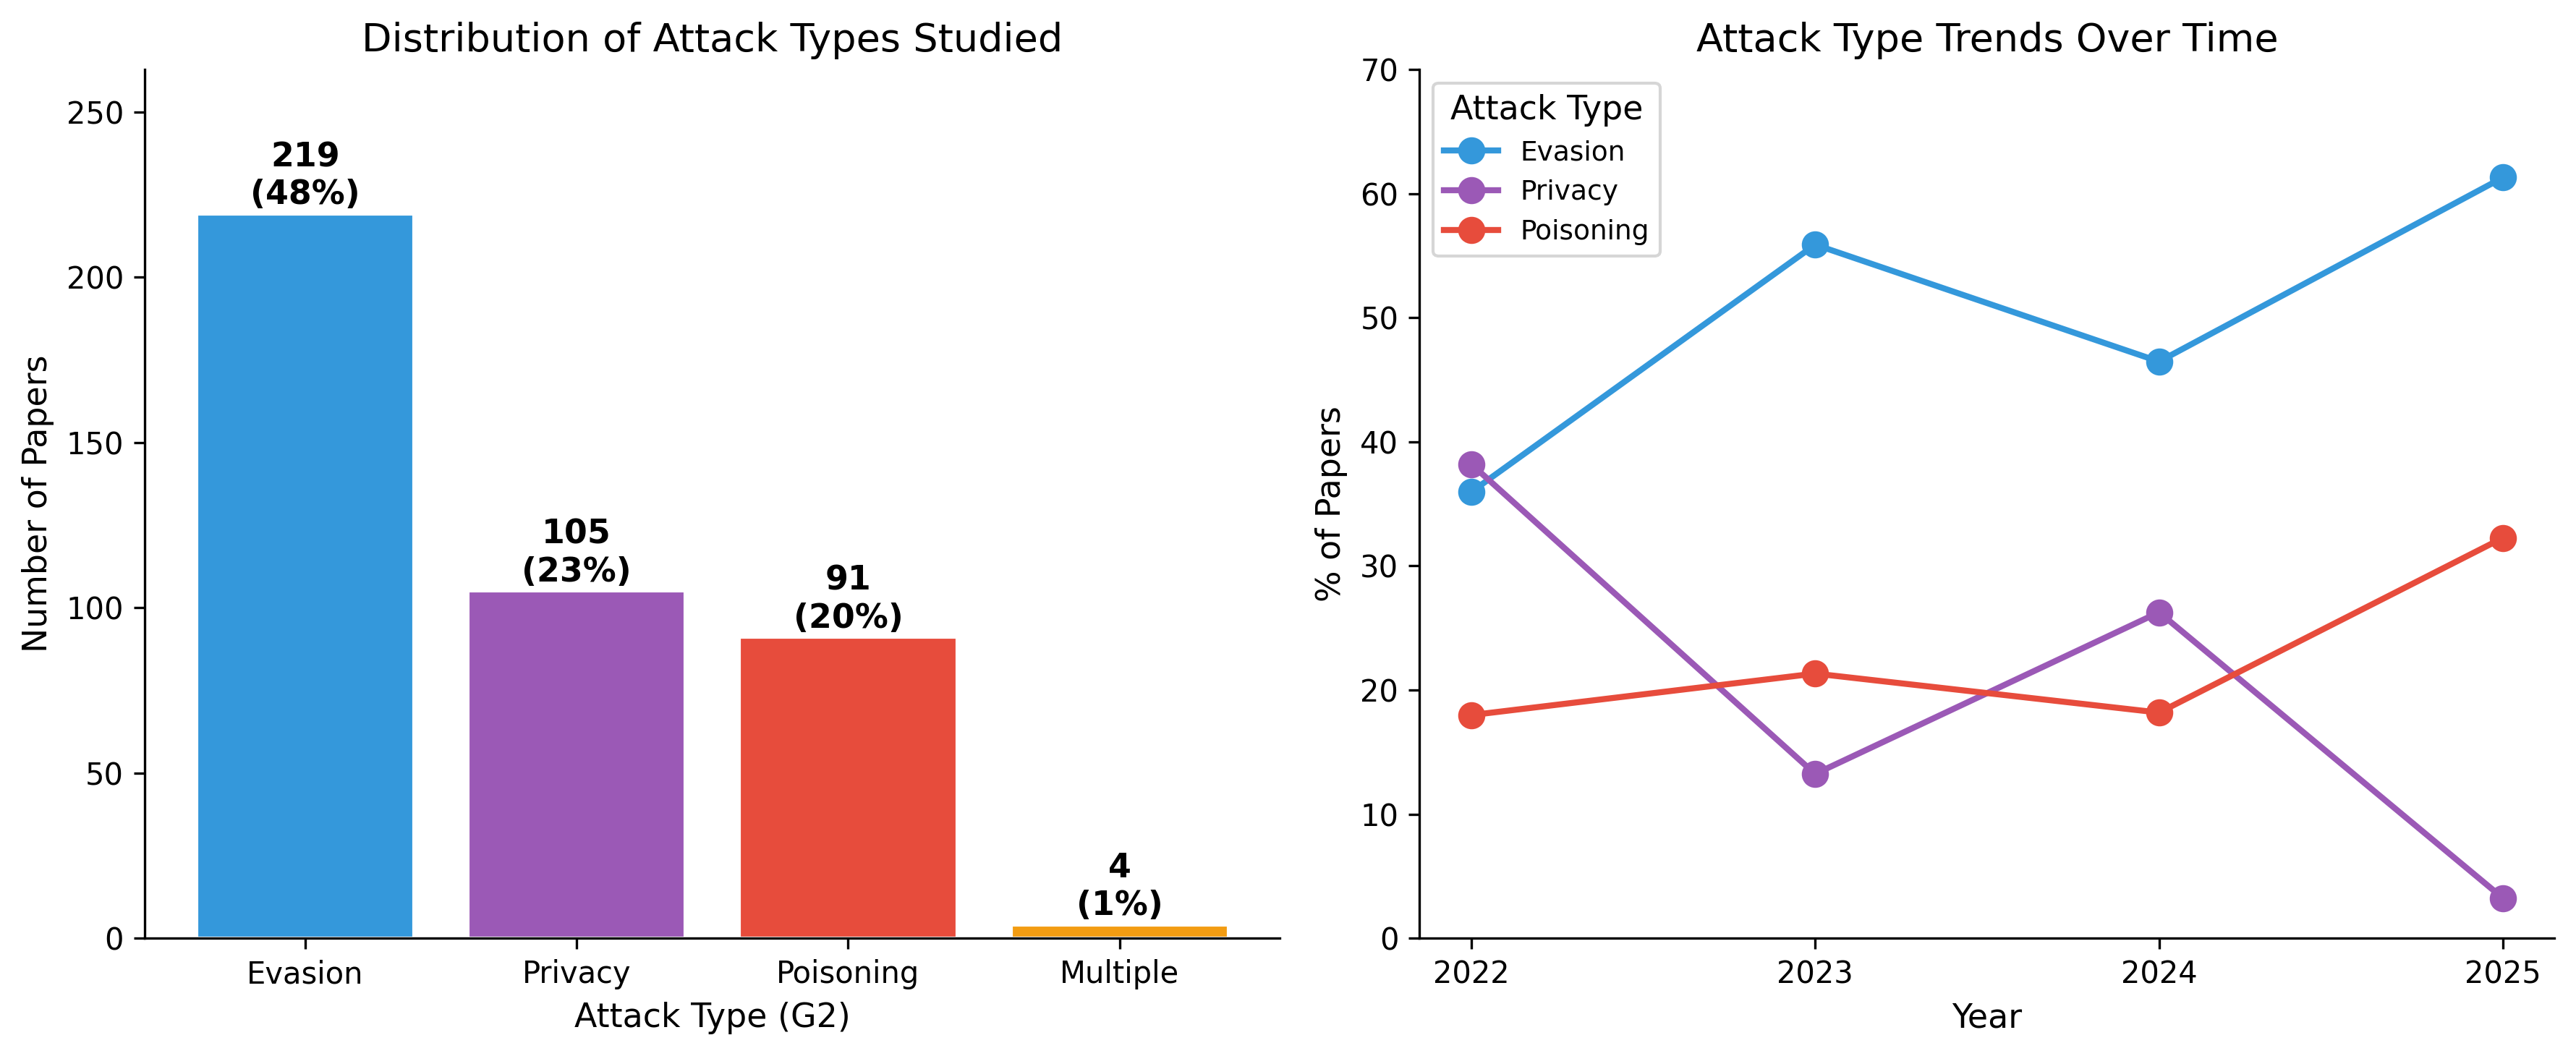
\includegraphics[width=0.9\textwidth]{fig07_attack_types.png}
    \caption{Attack type prevalence over 2022--2025. Evasion attacks remain most common, with poisoning/backdoor and privacy attacks gaining ground.}
    \label{fig:attack_types}
\end{figure}

Beyond aggregate statistics, we observed recurring qualitative patterns illuminating how the theory-practice gap manifests.

\paragraph{Utility versus robustness trade-offs.}
Many defenses exchange robustness for accuracy, latency, or usability. PatchCleanser and PatchCure~\citep{xiang2022patchcleanser, xiang2024patchcure} provide provable protection against adversarial patches but introduce processing overhead. Ahmed et al.~\citep{ahmed2022keyword} observed that voice interface defenses can reduce responsiveness. Privacy-preserving training methods can degrade model utility~\citep{liu2022mldoctor, tang2022membership}. Recent work including MIST~\citep{li2024mist} and CAMP~\citep{wang2025camp} reports robustness improvements with reduced utility costs.

\paragraph{Evaluation methodology and realism.}
A growing body of work emphasizes that conventional metrics may misrepresent security-relevant risk. Carlini et al.~\citep{carlini2022membership} argue that privacy evaluations should focus on extremely low false-positive rates and worst-case rather than average-case behavior. Human-centered evaluations reveal additional complexity: Ma et al.~\citep{ma2024avara} used virtual-reality driving experiments and found that perturbations deemed small under $L_p$ norms can remain perceptible or behaviorally relevant. These findings motivate evaluations incorporating adaptive attacks, explicit cost reporting, and human perception studies where appropriate.

\paragraph{Physical deployment and system integration.}
End-to-end settings introduce failure modes absent from isolated model testing. Research has moved robustness evaluation into physical and system-level contexts including autonomous driving and sensing~\citep{jia2022physical, cao2023lidar, kobayashi2025shadow}, medical imaging~\citep{liu2023xadv}, acoustic systems~\citep{ahmed2023tubes}, and content moderation primitives~\citep{zhang2025atkscopes}. This work also highlights pipeline interactions: Debenedetti et al.~\citep{debenedetti2024privacy} showed that filtering sensitive information can create privacy side channels, Nasr et al.~\citep{nasr2025magika} demonstrated evasion through file-type manipulation, and Chen et al.~\citep{chen2023obsan} reported cases where defensive transformations fail to survive compilation.

\paragraph{Attack and defense evolution.}
Recent attacks increasingly target persistence, system interactions, and emerging modalities. Hallyburton et al.~\citep{hallyburton2022frustum} exploit sensor fusion in autonomous systems. Prompt-based LLM attacks are automated by methods such as PAIR~\citep{chao2023jailbreaking} and TAP~\citep{mehrotra2024tree}. Cross-modal exploits can jailbreak vision-language models via images~\citep{qi2024visual}. Backdoors designed for persistence survive model merging~\citep{wang2025mergebackdoor} and continual learning~\citep{guo2025persistent}. Defenses have become more context-aware, including Blacklight for detecting query patterns~\citep{li2022blacklight}, JBShield for intervening in jailbreak dynamics~\citep{zhang2025jbshield}, and SafeSpeech for degrading voice-cloning data~\citep{zhang2025safespeech}.

\paragraph{Economic and organizational factors.}
A smaller subset of papers addresses attacker and defender incentives. Cong et al.~\citep{cong2022sslguard} note that stealing self-supervised models can be inexpensive relative to training costs. Lu et al.~\citep{lu2024neural} show that watermark removal requires only modest resources. On deployment, Mink et al.~\citep{mink2023barriers} document unclear ownership of adversarial risk and limited capacity to integrate adversarial testing into development cycles. These findings highlight needs for usable tooling, clearer responsibility boundaries, and incentives rewarding security-oriented evaluation.

%==============================================================================
% 7. EMERGING CHALLENGES IN FOUNDATION MODELS
%==============================================================================
\section{Emerging Challenges in Foundation Models}

The proliferation of large language models and multimodal foundation models during 2022--2025 has introduced adversarial challenges that parallel but also diverge from those in traditional ML. These systems process discrete tokens, accept multimodal inputs, and are typically deployed through rate-limited APIs.

\subsection{Jailbreaking Attacks}

Early adversarial behaviors manifested as ``jailbreaks,'' where users discovered that specific prompt formulations could elicit content violating model policies. Research subsequently developed automated jailbreak generation methods.

Zou et al.~\citep{zou2023universal} introduced the Greedy Coordinate Gradient (GCG) attack, which optimizes adversarial suffixes through gradient-based discrete token search. GCG demonstrated transferability to black-box systems including ChatGPT and Claude, though it requires white-box access to an open-source model for suffix generation. The accompanying AdvBench benchmark has become standard for evaluating jailbreak attacks.

Liu et al.~\citep{liu2024autodan} proposed AutoDAN, using hierarchical genetic algorithms to generate semantically meaningful jailbreak prompts that evade perplexity-based detection. Unlike GCG's nonsensical suffixes, AutoDAN produces readable adversarial text.

Chao et al.~\citep{chao2023jailbreaking} developed PAIR (Prompt Automatic Iterative Refinement), achieving jailbreaks with approximately 20 queries by using an attacker LLM to iteratively refine prompts. This black-box approach substantially reduces query requirements compared to optimization-based methods.

Mehrotra et al.~\citep{mehrotra2024tree} introduced TAP (Tree of Attacks with Pruning), using tree-of-thought reasoning to explore attack strategies while pruning unpromising branches. TAP achieves high success rates with further reduced query counts.

For standardized evaluation, Mazeika et al.~\citep{mazeika2024harmbench} developed HarmBench, comparing 18 red-teaming methods across 33 LLMs. Their R2D2 defense, based on adversarial training with generated attacks, achieves improved robustness compared to baseline aligned models.

\subsection{Prompt Injection}

Prompt injection attacks manipulate LLM behavior by embedding malicious instructions in user-provided or retrieved content. Liu et al.~\citep{liu2024prompt} provided the first formal framework and benchmark, evaluating five attack strategies and ten defenses across multiple LLMs and application scenarios.

Indirect prompt injection poses particular challenges for LLM-integrated applications. When models process external content (web pages, documents, emails), attackers can embed instructions that execute when the content is retrieved. Greshake et al.~\citep{greshake2023youve} demonstrated such attacks against retrieval-augmented systems, while Zhan et al.~\citep{zhan2024injecagent} showed that agentic systems with tool access face amplified risks.

\subsection{Multimodal Attacks}

Vision-language models introduce cross-modal attack surfaces. Qi et al.~\citep{qi2024visual} demonstrated that adversarial images can trigger harmful text generation, bypassing text-only safety measures. Gong et al.~\citep{gong2024figstep} showed that encoding harmful text as images circumvents text-based content filters.

These multimodal vulnerabilities complicate defense design, as safety measures must address threats across all input modalities and their interactions.

\subsection{Defenses and Alignment}

Defense strategies for LLMs span multiple approaches. Input and output filtering attempts to detect and block harmful content. Specialized models such as LlamaGuard~\citep{inan2023llamaguard} and frameworks like NeMo Guardrails~\citep{rebedea2023nemo} provide structured safety layers. Automated red-teaming frameworks~\citep{bertrand2024rainbow, hong2024curiosity} enable systematic vulnerability discovery.

Alignment techniques including Constitutional AI~\citep{bai2022constitutional} and reinforcement learning from human feedback aim to instill safety properties during training. However, these measures exhibit brittleness: homoglyphs, encoding tricks, and indirect injection can circumvent filters, while aligned models remain vulnerable to sophisticated jailbreaks.

\subsection{Implications for the Theory-Practice Gap}

LLM security research exhibits distinctive characteristics relevant to the theory-practice gap. The most effective automated attacks often require white-box gradient access or substantial queries, yet commercial APIs provide only black-box access with rate limits. Deployed models receive frequent updates, potentially invalidating discovered vulnerabilities. Defining adversarial success is more subjective than for classifiers, making evaluation inherently challenging.

Foundation models also pose systemic risks because vulnerabilities in widely-deployed base models can propagate across numerous downstream applications~\citep{bommasani2021opportunities}. Addressing these challenges will require collaboration across ML, security, and human-computer interaction communities, integrating perspectives on system design, threat modeling, and user behavior.

%==============================================================================
% 8. TEMPORAL TRENDS
%==============================================================================
\section{Temporal Trends}

\begin{figure}[H]
    \centering
    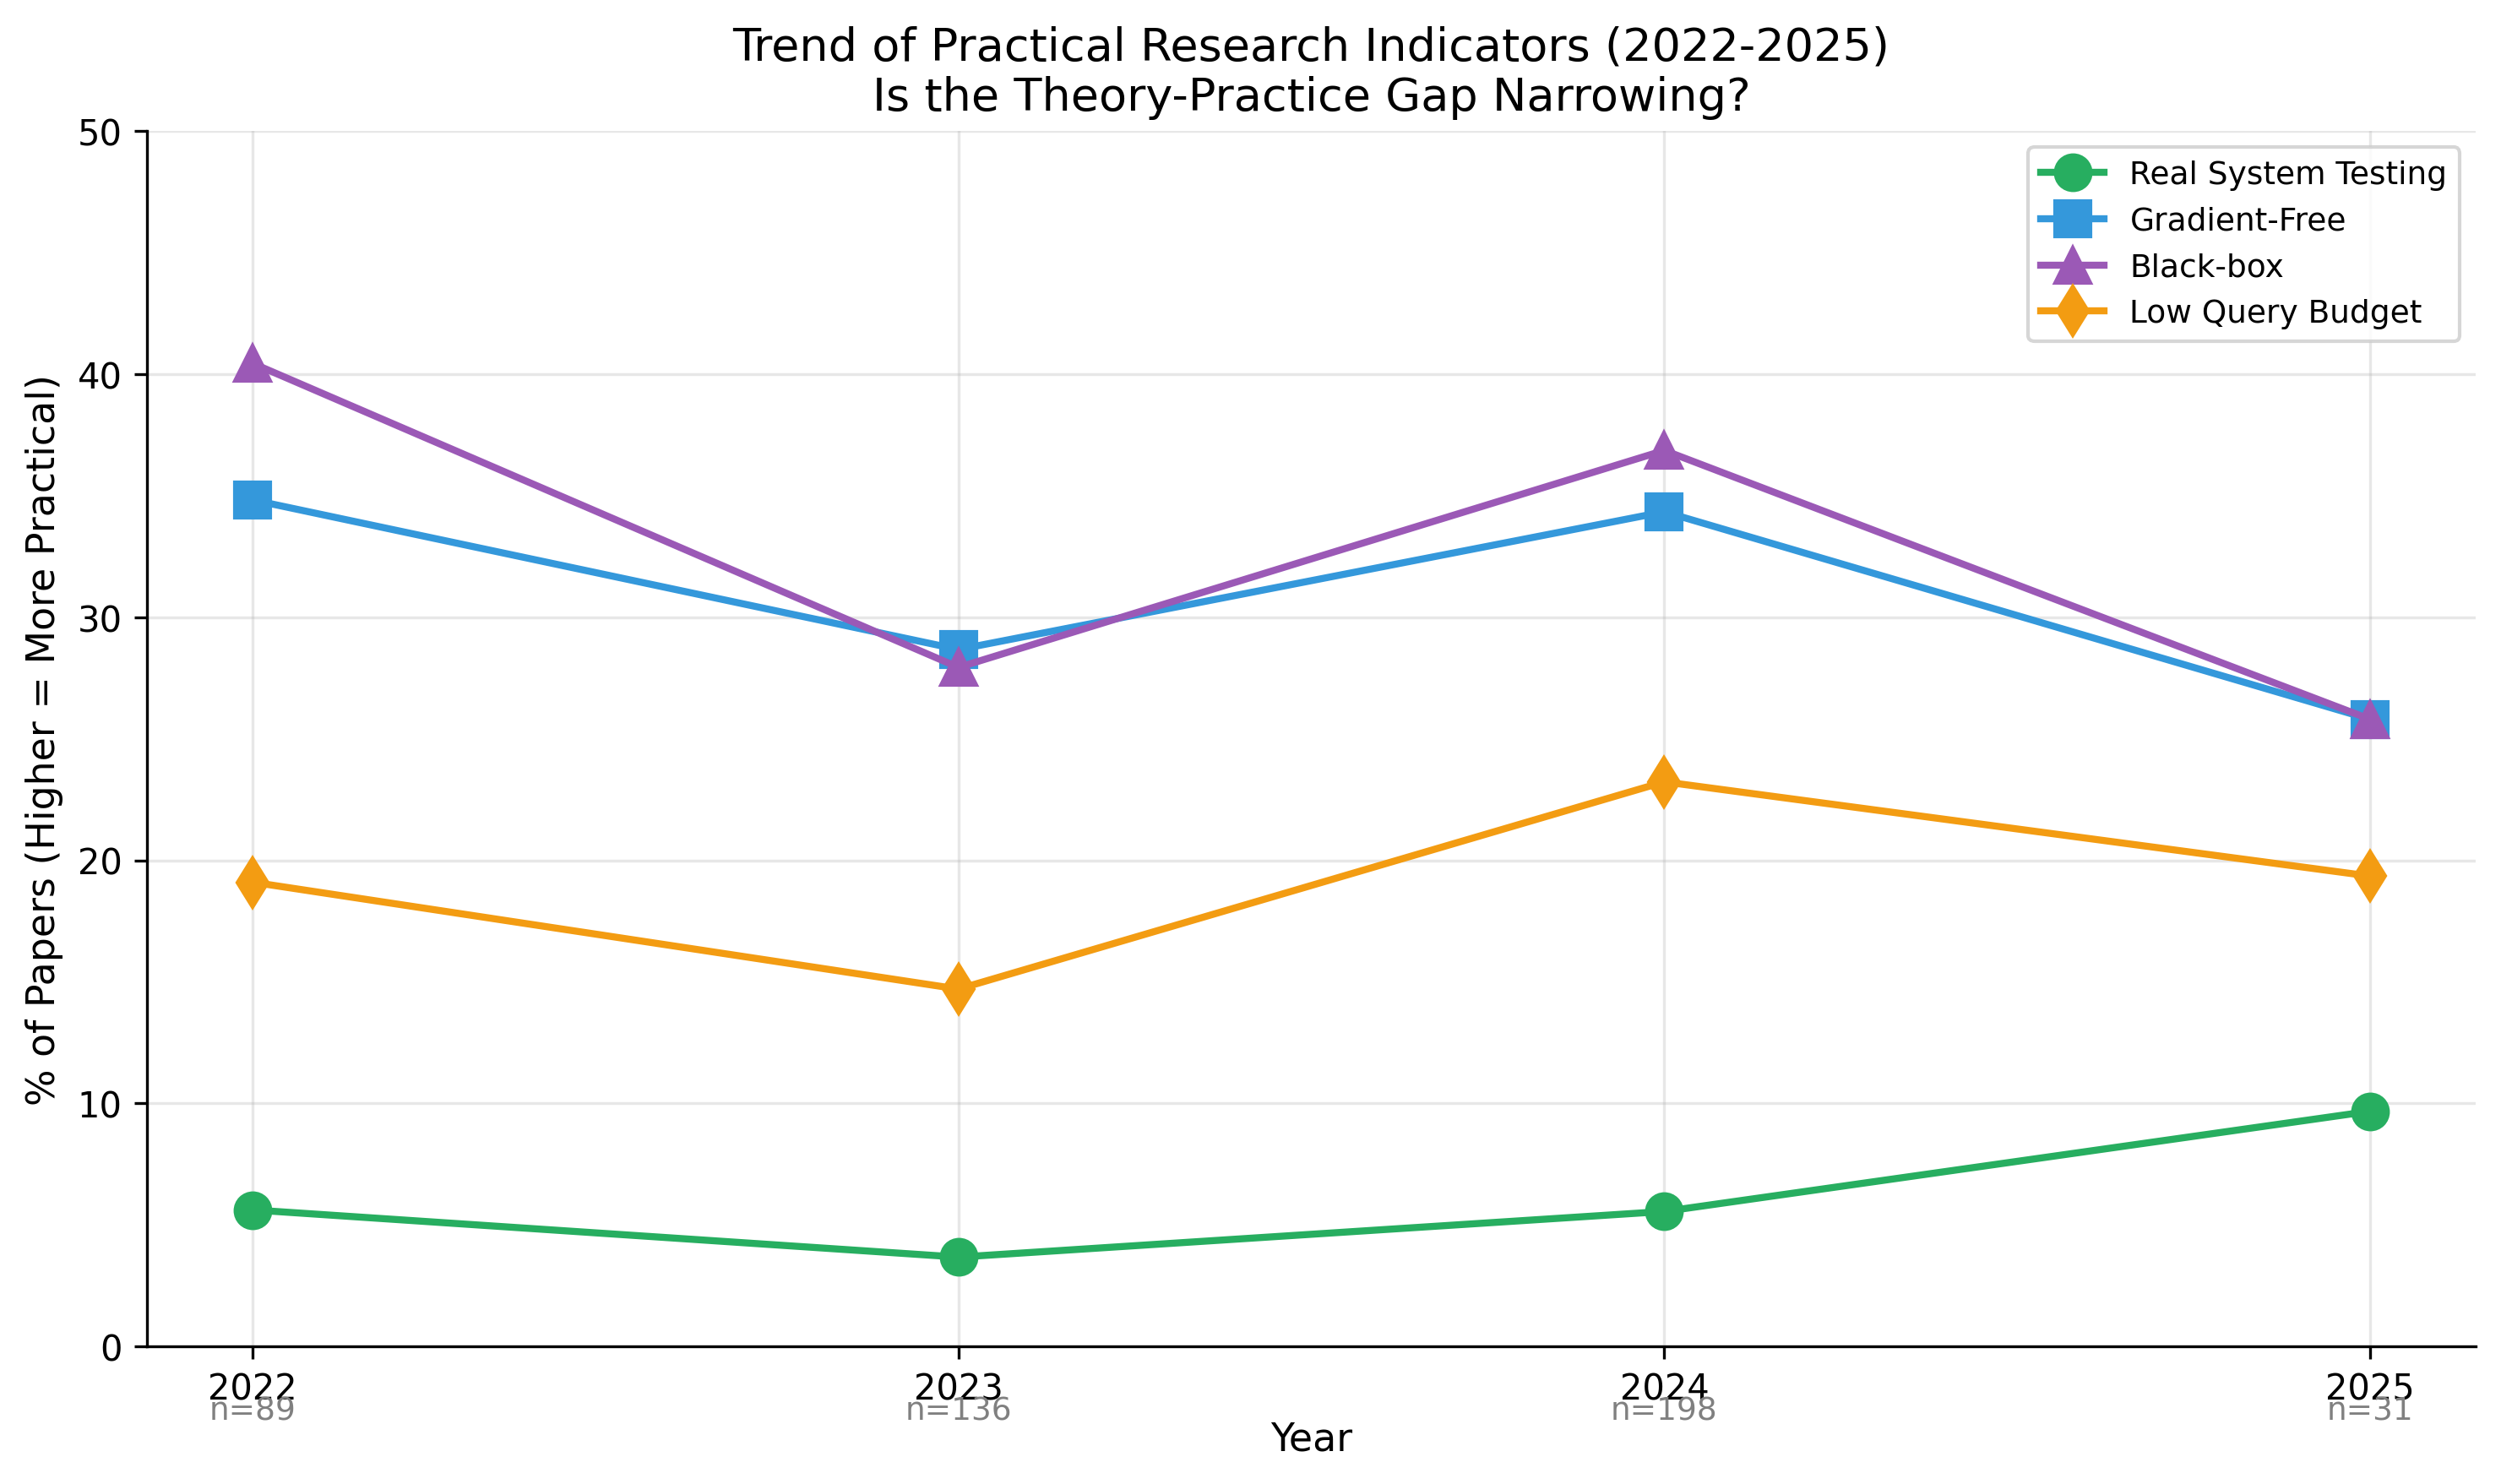
\includegraphics[width=0.9\textwidth]{fig11_yearly_trends.png}
    \caption{Trends from 2022 to 2025 on key gap indicators.}
    \label{fig:trends}
\end{figure}

Figure~\ref{fig:trends} summarizes how indicators evolved following the critique of Apruzzese et al.~\citep{apruzzese2022real}.

\begin{itemize}[noitemsep]
    \item \textbf{Real-world testing} remained near 5\% throughout, with no clear upward trend.
    \item \textbf{Gradient dependency} stayed high at approximately two-thirds of papers, with only modest decrease by early 2025.
    \item \textbf{White-box threat models} remained dominant, hovering around 60--64\%.
    \item \textbf{High query budgets} declined slightly from approximately 80\% in 2022--2023 to the mid-to-high 70\% range by 2025.
    \item \textbf{Attack-type composition} shifted, with poisoning/backdoor and privacy work increasing by 2024--2025.
    \item \textbf{Modalities} broadened modestly, with text and multimodal work increasing in 2024 as LLM security topics entered venue pipelines.
    \item \textbf{Economics/organizational discussion} remained low at approximately 10--12\% without meaningful increase.
\end{itemize}

Overall, the data show limited movement on core gap indicators through early 2025, alongside gradual broadening of research topics and modalities.

%==============================================================================
% 9. CROSS-VENUE ANALYSIS
%==============================================================================
\section{Cross-Venue Analysis}

\begin{figure}[H]
    \centering
    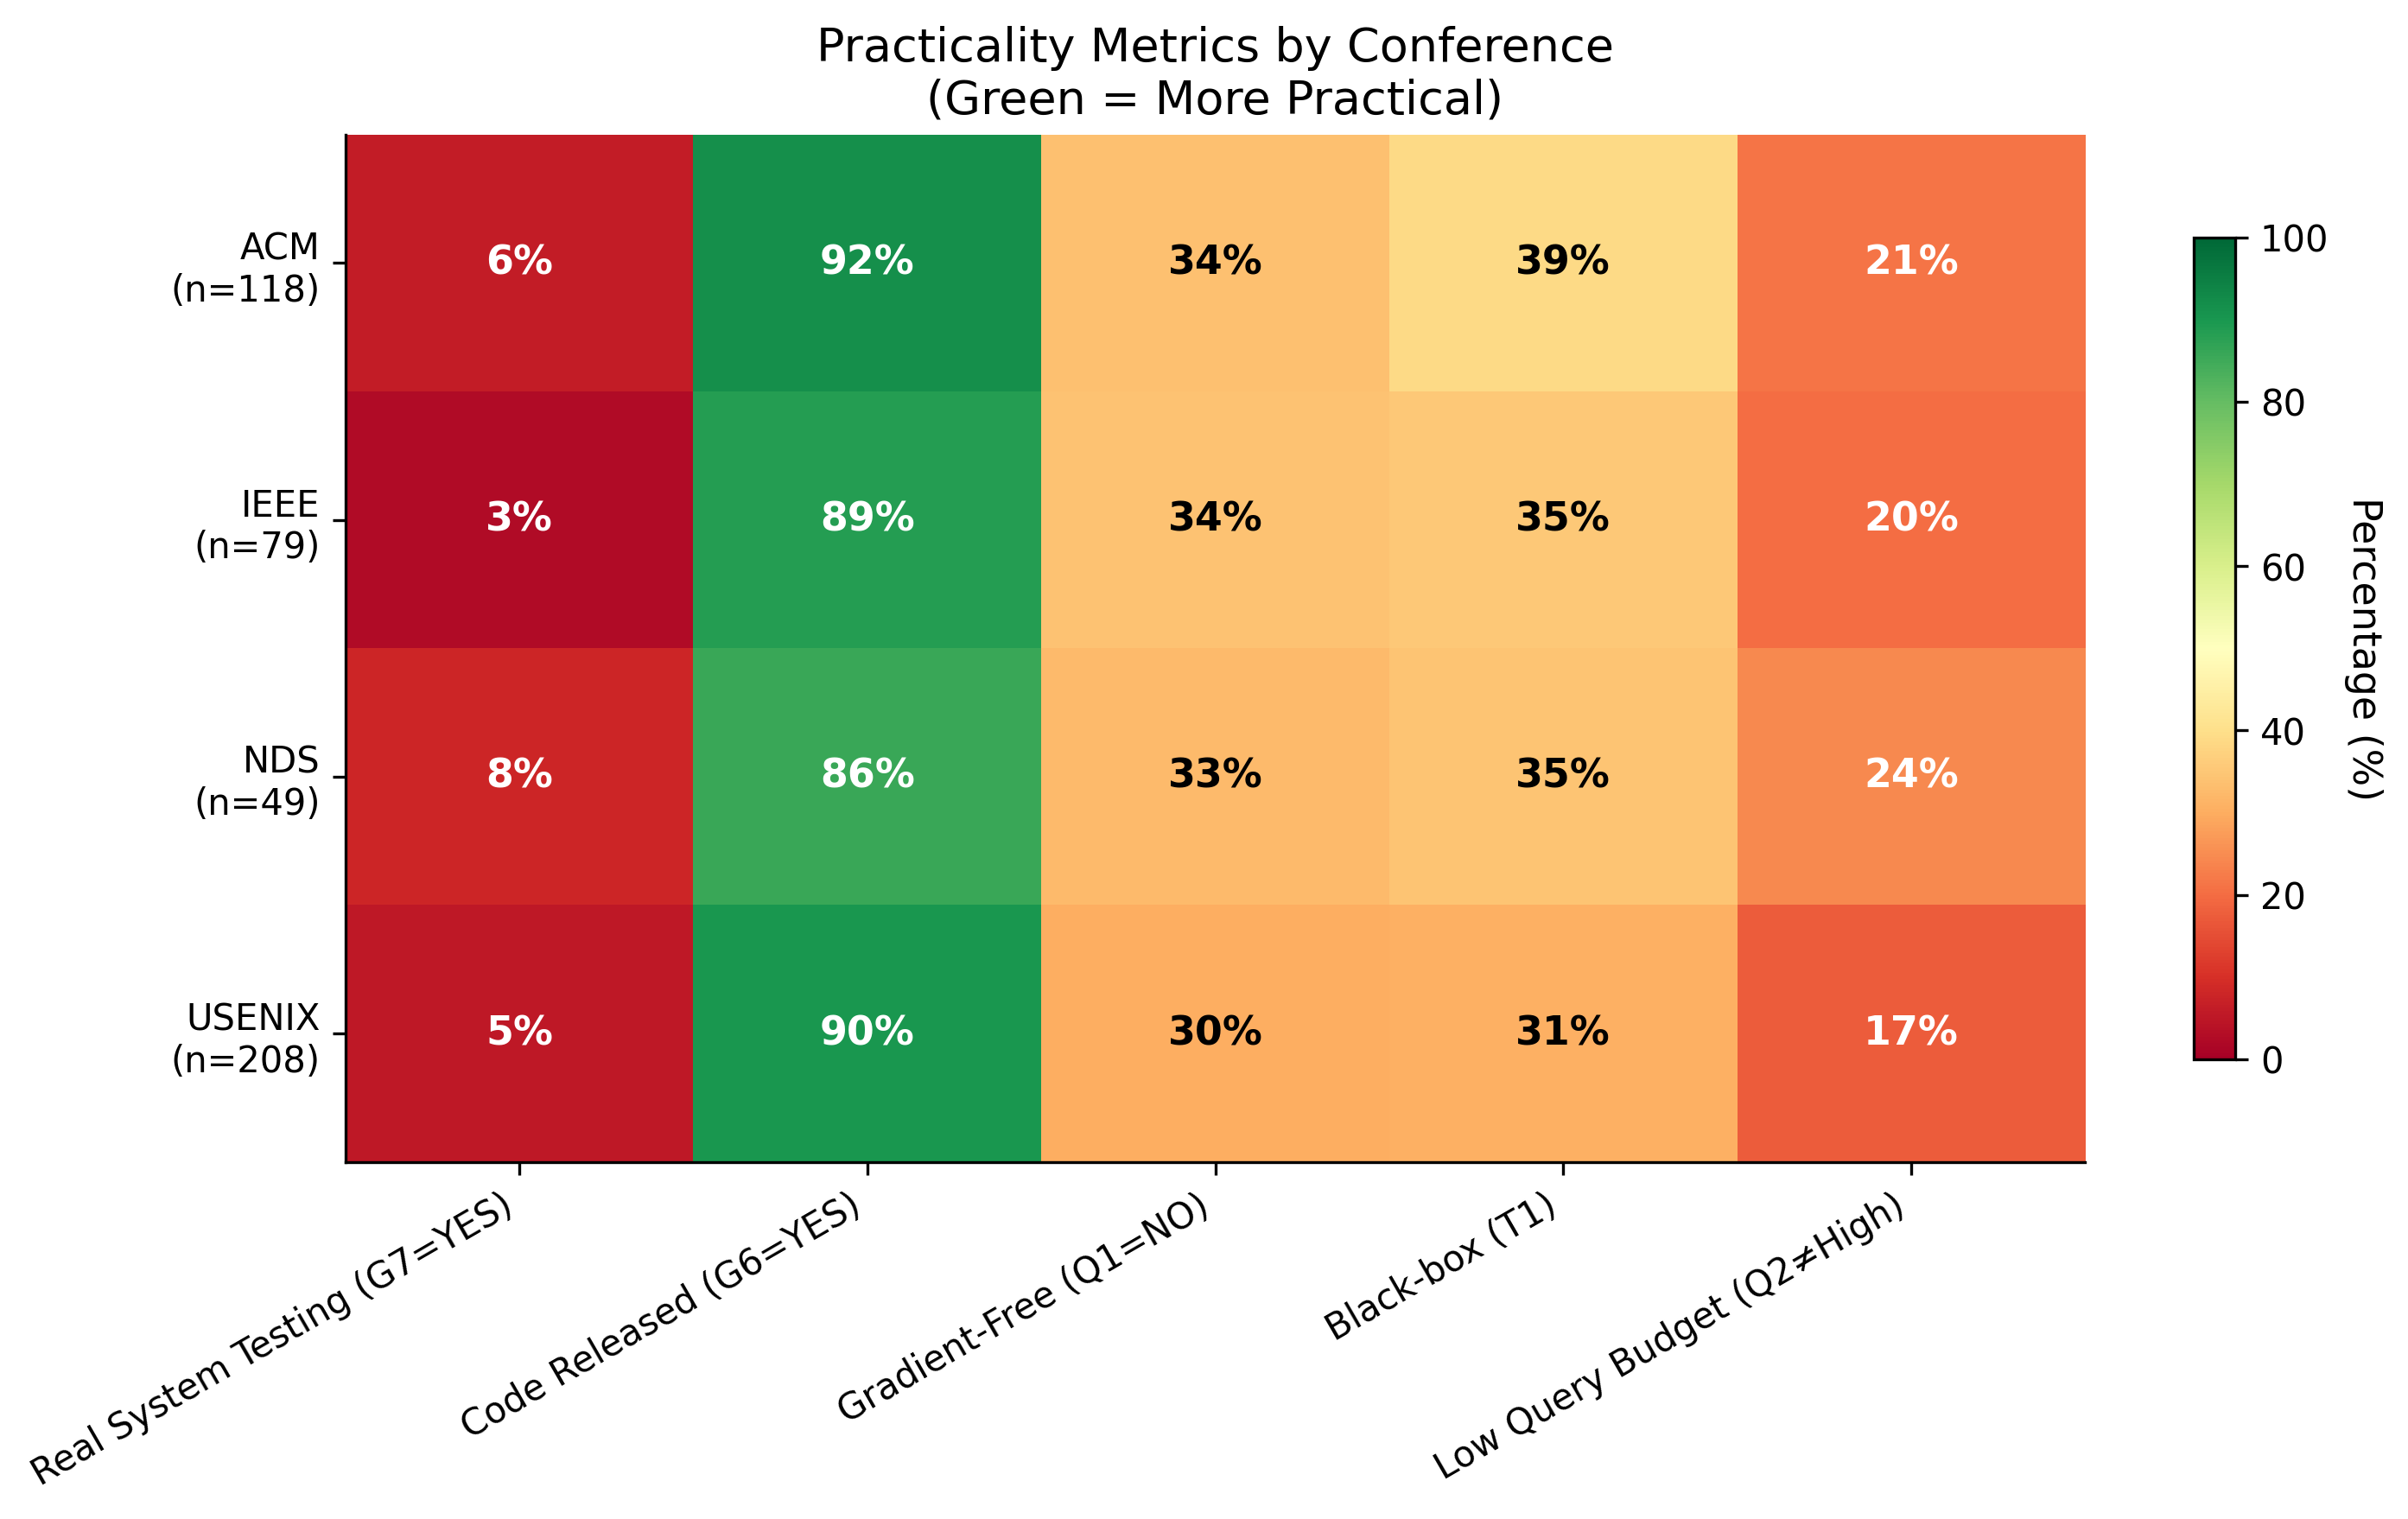
\includegraphics[width=0.9\textwidth]{fig10_conference_comparison.png}
    \caption{Comparison of adversarial ML research characteristics by conference.}
    \label{fig:heatmap}
\end{figure}

While all four venues exhibited similar overall patterns, each demonstrated distinct emphases.

CCS papers frequently situated adversarial ML within broader systems and business contexts, addressing model theft, watermarking, and human factors. S\&P publications tended toward formal or measurement-driven approaches, featuring systematic evaluations and systematization-of-knowledge papers with explicit threat model justification. NDSS papers, though fewer, often explored specific systems or emerging applications including physical-world attacks and federated learning, grounding evaluations in realistic settings. USENIX contributed the largest paper volume across diverse topics; several tested attacks or defenses on real platforms and released implementation artifacts.

Comparing attack- and defense-oriented papers, defense papers were marginally more likely to assume black-box access or avoid gradient dependence, with slightly higher real-system testing rates. Nonetheless, only a small minority conducted deployed evaluations across all categories.

The venues complement each other: CCS and NDSS emphasize system integration and context, S\&P provides formal rigor, and USENIX encourages empirical testing. All would benefit from stronger focus on practical deployment and domain diversification.

%==============================================================================
% 10. RECOMMENDATIONS
%==============================================================================
\section{Recommendations}

To narrow the gap between academic research and operational requirements, we offer stakeholder-specific recommendations.

\paragraph{For researchers: prioritize realistic assumptions and evaluations.}
Where feasible, validate methods under deployment-like conditions including limited queries, partial knowledge, pipeline effects, and realistic computational constraints. When white-box access or large query budgets are assumed, explicitly justify how attackers could plausibly obtain them. For defenses, evaluate against adaptive adversaries and report utility costs including accuracy, latency, and user experience alongside robustness metrics. Incorporate human-centered evaluation of perceptibility where relevant, and document system-level assumptions clearly.

\paragraph{For conference organizers and reviewers: reward practical relevance.}
Review criteria can more explicitly assess threat model realism and deployment constraints, even when live-system testing is infeasible. Conferences can incentivize practical work through artifact evaluation policies and recognition for deployed evaluations. Dedicated tracks, sessions, or workshops focusing on industry constraints and end-to-end robustness can highlight this research direction.

\paragraph{For industry practitioners: share constraints and evaluation insights.}
Organizations deploying ML systems can log and share (where possible with appropriate anonymization) adversarial incidents and unusual inputs reflecting operational threat surfaces. Partnerships with researchers through limited testing access, red teaming, or structured disclosure programs can ground academic work in realistic constraints. Practitioners should evaluate proposed defenses under their own threat models and cost constraints rather than adopting benchmark-reported robustness at face value.

For LLM deployments specifically, we recommend sandboxing tool access, treating external content as untrusted with appropriate sanitization, implementing rate limiting and anomaly detection for automated queries, providing user education about indirect prompt injection risks, and maintaining incident response procedures for adversarial failures.

\paragraph{For funders and the broader community: support bridging infrastructure.}
Funding mechanisms can encourage academia-industry collaboration enabling evaluation on real systems with realistic data. Community benchmarks and competitions can incorporate operational constraints including low-query attacks, API-only access, and cost-aware defenses. Interdisciplinary collaboration spanning security, human-computer interaction, and policy can align threat models, evaluation metrics, and adoption pathways.

%==============================================================================
% 11. LIMITATIONS AND THREATS TO VALIDITY
%==============================================================================
\section{Limitations and Threats to Validity}

This study has several limitations. Our focus on four security conferences means observations may not reflect adversarial ML research in machine learning venues or other domains with different norms. The coding framework and Gap Score simplify complex realities through binary flags and equal weighting; these heuristics cannot capture partial progress or nuanced threat models. Classification was performed by the authors, which may introduce bias or overlook subtle distinctions.

The field evolves rapidly; our dataset ends in early 2025, and the distribution of research may shift as work on large language models and other modalities expands. What constitutes ``practical'' is context-dependent and may change as technology and attacker capabilities evolve; assumptions impractical today might become realistic in the future.

Despite these caveats, we believe this synthesis of quantitative trends and qualitative themes provides useful orientation for researchers and practitioners seeking to understand the current state of adversarial ML research and its relationship to deployment realities.

%==============================================================================
% 12. CONCLUSION
%==============================================================================
\section{Conclusion}

Our review of 454 adversarial ML papers published from 2022 through 2025 reveals that the field has grown in technical sophistication while beginning to engage more seriously with practical considerations. Approximately one study in twenty evaluated methods on deployed systems, and many continued to assume white-box access, gradient information, or generous query budgets. These simplifications are understandable given the complexity of real deployments but highlight where future work can focus.

Beyond quantitative gaps, we observed qualitative mismatches: standard benchmarks emphasize $L_p$ norms and worst-case analysis rather than factors more relevant to practitioners such as human perception, system integration, and economic cost. Nevertheless, encouraging trends are evident, including increased code release, emerging research on query-efficient and gradient-free methods, and growing discourse on realistic threat modeling alongside economic and human factors.

To align adversarial ML research with real-world challenges, the community should emphasize realistic threat models, constrained attacker access, production system testing, domain diversification beyond computer vision, and consideration of human and economic factors. Coordinated efforts across researchers, conferences, practitioners, and funders can accelerate progress: validating methods under deployment conditions, incorporating practical relevance in peer review, sharing evaluation data and insights, and supporting collaborative projects bridging theory and practice. Ensuring AI system robustness as these systems proliferate across high-stakes domains represents a societal imperative, and increased awareness and collaboration can help narrow the gap between adversarial ML research and operational security.

%==============================================================================
% REFERENCES
%==============================================================================
\newpage
\bibliographystyle{unsrtnat}
\bibliography{ref}

%==============================================================================
% APPENDIX
%==============================================================================
\newpage
\appendix
\section{Complete Paper Analysis Dataset}

For transparency and to facilitate future meta-analyses, we provide our full dataset of coded results for all 454 papers in the supplementary material (\texttt{all\_conferences\_analysis\_results\_2022\_2025.csv}). Table~\ref{tab:full_dataset_summary} shows a condensed excerpt of key fields.

The dataset columns include:
\begin{itemize}[noitemsep]
    \item Year, Conference, Title (first author and shorthand)
    \item G1 (Focus: attack or defense), G2 (Attack Type: Evasion, Poison, Privacy, Multiple)
    \item G3 (ML paradigm: DL=deep learning, Trad=traditional ML, Both)
    \item G4 (Data Domain: Images, Text, Audio, Malware, Other)
    \item G5 (Economics discussed: YES/NO)
    \item G6 (Code released: YES/NO)
    \item G7 (Real system testing: YES/NO)
    \item T1 (Threat model: White-box, Gray-box, Black-box)
    \item T2 (Training data access assumed: Full, Partial, None)
    \item Q1 (Requires gradients: YES/NO)
    \item Q2 (Query budget: High, Low, None)
    \item Q3 (Computation needed: High = GPU or extensive, Low = CPU or minimal)
    \item Gap Score (0--6) as defined in the paper.
\end{itemize}

In the table, binary fields are indicated with checkmarks (Yes) or \(\times\) (No), and abbreviated labels are used for threat model (W = white, B = black, G = gray) and other categorical fields for compactness.

\begin{landscape}
\begin{tiny}
\setlength{\tabcolsep}{0.65pt}
\renewcommand{\arraystretch}{0.7}
\begin{longtable}{|p{0.7cm}|p{0.9cm}|p{1.4cm}|p{0.7cm}|p{1.0cm}|p{0.7cm}|p{0.7cm}|p{0.7cm}|p{0.7cm}|p{0.7cm}|p{0.7cm}|p{0.7cm}|p{0.7cm}|p{0.7cm}|p{0.7cm}|p{0.7cm}|p{0.7cm}|}
\caption{Summary of all reviewed papers with key taxonomy fields. (G1: Focus; G2: Attack Type; G3: ML Type; G4: Domain; G5: Economics; G6: Code; G7: Real-world eval; T1: Threat Model; T2: Training Data Access; Q1: Gradient; Q2: Query Budget; Q3: Computation; WB: White-box flag; Gap Score.)}\label{tab:full_dataset_summary}\\
\hline
Year & Venue & First Author & G1 & G2 & G3 & G4 & G5 & G6 & G7 & T1 & T2 & Q1 & Q2 & Q3 & WB & Gap \\
\hline
\endfirsthead
\hline
Year & Venue & First Author & G1 & G2 & G3 & G4 & G5 & G6 & G7 & T1 & T2 & Q1 & Q2 & Q3 & WB & Gap \\
\hline
\endhead
\hline
\multicolumn{17}{r}{\small (Continued on next page)}\\
\hline
\endfoot
\hline
\endlastfoot
\csvreader[
    separator=semicolon,
    late after line=\\\hline
]{all_conferences_analysis_results_clean.csv}{
Year=\Year,
Conference=\Conference,
Authors=\Authors,
G1=\GOne,
G2=\GTwo,
G3=\GThree,
G4=\GFour,
G5=\GFive,
G6=\GSix,
G7=\GSeven,
T1=\Tone,
T2=\Ttwo,
Q1=\Qone,
Q2=\Qtwo,
Q3=\Qthree,
Flag_WB=\FWB,
Traditional_Score=\TScore
}{
\Year & \Conference & \StrBefore{\Authors}{ } & \GOne & \IfStrEq{\GTwo}{Evasion}{Ev}{\IfStrEq{\GTwo}{Poisoning}{Po}{\IfStrEq{\GTwo}{Privacy}{Pr}{\IfStrEq{\GTwo}{Multiple}{M}{\GTwo}}}} & \GThree & \IfStrEq{\GFour}{Images}{Img}{\IfStrEq{\GFour}{Text}{Txt}{\IfStrEq{\GFour}{Audio}{Aud}{\IfStrEq{\GFour}{Malware}{Mal}{Oth}}}} & \yn{\GFive} & \yn{\GSix} & \yn{\GSeven} & \threat{\Tone} & \access{\Ttwo} & \yn{\Qone} & \level{\Qtwo} & \level{\Qthree} & \yn{\FWB} & \TScore
}
\end{longtable}
\end{tiny}
\end{landscape}

\end{document}